\documentclass[twoside]{book}

% Packages required by doxygen
\usepackage{fixltx2e}
\usepackage{calc}
\usepackage{doxygen}
\usepackage[export]{adjustbox} % also loads graphicx
\usepackage{graphicx}
\usepackage[utf8]{inputenc}
\usepackage{makeidx}
\usepackage{multicol}
\usepackage{multirow}
\PassOptionsToPackage{warn}{textcomp}
\usepackage{textcomp}
\usepackage[nointegrals]{wasysym}
\usepackage[table]{xcolor}

% Font selection
\usepackage[T1]{fontenc}
\usepackage[scaled=.90]{helvet}
\usepackage{courier}
\usepackage{amssymb}
\usepackage{sectsty}
\renewcommand{\familydefault}{\sfdefault}
\allsectionsfont{%
  \fontseries{bc}\selectfont%
  \color{darkgray}%
}
\renewcommand{\DoxyLabelFont}{%
  \fontseries{bc}\selectfont%
  \color{darkgray}%
}
\newcommand{\+}{\discretionary{\mbox{\scriptsize$\hookleftarrow$}}{}{}}

% Page & text layout
\usepackage{geometry}
\geometry{%
  a4paper,%
  top=2.5cm,%
  bottom=2.5cm,%
  left=2.5cm,%
  right=2.5cm%
}
\tolerance=750
\hfuzz=15pt
\hbadness=750
\setlength{\emergencystretch}{15pt}
\setlength{\parindent}{0cm}
\setlength{\parskip}{3ex plus 2ex minus 2ex}
\makeatletter
\renewcommand{\paragraph}{%
  \@startsection{paragraph}{4}{0ex}{-1.0ex}{1.0ex}{%
    \normalfont\normalsize\bfseries\SS@parafont%
  }%
}
\renewcommand{\subparagraph}{%
  \@startsection{subparagraph}{5}{0ex}{-1.0ex}{1.0ex}{%
    \normalfont\normalsize\bfseries\SS@subparafont%
  }%
}
\makeatother

% Headers & footers
\usepackage{fancyhdr}
\pagestyle{fancyplain}
\fancyhead[LE]{\fancyplain{}{\bfseries\thepage}}
\fancyhead[CE]{\fancyplain{}{}}
\fancyhead[RE]{\fancyplain{}{\bfseries\leftmark}}
\fancyhead[LO]{\fancyplain{}{\bfseries\rightmark}}
\fancyhead[CO]{\fancyplain{}{}}
\fancyhead[RO]{\fancyplain{}{\bfseries\thepage}}
\fancyfoot[LE]{\fancyplain{}{}}
\fancyfoot[CE]{\fancyplain{}{}}
\fancyfoot[RE]{\fancyplain{}{\bfseries\scriptsize Generated by Doxygen }}
\fancyfoot[LO]{\fancyplain{}{\bfseries\scriptsize Generated by Doxygen }}
\fancyfoot[CO]{\fancyplain{}{}}
\fancyfoot[RO]{\fancyplain{}{}}
\renewcommand{\footrulewidth}{0.4pt}
\renewcommand{\chaptermark}[1]{%
  \markboth{#1}{}%
}
\renewcommand{\sectionmark}[1]{%
  \markright{\thesection\ #1}%
}

% Indices & bibliography
\usepackage{natbib}
\usepackage[titles]{tocloft}
\setcounter{tocdepth}{3}
\setcounter{secnumdepth}{5}
\makeindex

% Hyperlinks (required, but should be loaded last)
\usepackage{ifpdf}
\ifpdf
  \usepackage[pdftex,pagebackref=true]{hyperref}
\else
  \usepackage[ps2pdf,pagebackref=true]{hyperref}
\fi
\hypersetup{%
  colorlinks=true,%
  linkcolor=blue,%
  citecolor=blue,%
  unicode%
}

% Custom commands
\newcommand{\clearemptydoublepage}{%
  \newpage{\pagestyle{empty}\cleardoublepage}%
}

\usepackage{caption}
\captionsetup{labelsep=space,justification=centering,font={bf},singlelinecheck=off,skip=4pt,position=top}

%===== C O N T E N T S =====

\begin{document}

% Titlepage & ToC
\hypersetup{pageanchor=false,
             bookmarksnumbered=true,
             pdfencoding=unicode
            }
\pagenumbering{alph}
\begin{titlepage}
\vspace*{7cm}
\begin{center}%
{\Large M\+\_\+process }\\
\vspace*{1cm}
{\large Generated by Doxygen 1.8.14}\\
\end{center}
\end{titlepage}
\clearemptydoublepage
\pagenumbering{roman}
\tableofcontents
\clearemptydoublepage
\pagenumbering{arabic}
\hypersetup{pageanchor=true}

%--- Begin generated contents ---
\chapter{M\+\_\+process Fortran Module}
\label{index}\hypertarget{index}{}\hypertarget{index_Introduction}{}\doxysection{Introduction}\label{index_Introduction}
procedures that call the C procedure popen(3c) using the intrinsic I\+S\+O\+\_\+\+C\+\_\+\+B\+I\+N\+D\+I\+NG module in order to allow reading and writing from a process from Fortran.

 
\chapter{Modules Index}
\section{Modules List}
Here is a list of all modules with brief descriptions\+:\begin{DoxyCompactList}
\item\contentsline{section}{\mbox{\hyperlink{namespacem__process}{m\+\_\+process}} \\*\subsubsection*{N\+A\+ME}

M\+\_\+process(3fm) -\/ \mbox{[}M\+\_\+process\mbox{]} Fortran Module for calling process-\/related C functions from Fortran (L\+I\+C\+E\+N\+SE\+:PD) }{\pageref{namespacem__process}}{}
\end{DoxyCompactList}

\chapter{Data Type Index}
\section{Data Types List}
Here are the data types with brief descriptions\+:\begin{DoxyCompactList}
\item\contentsline{section}{\mbox{\hyperlink{interfacem__process_1_1fflush}{m\+\_\+process\+::fflush}} \\*\subsubsection*{N\+A\+ME}

fflush(3fp) -\/ flush buffered file output \subsubsection*{S\+Y\+N\+O\+P\+S\+IS}}{\pageref{interfacem__process_1_1fflush}}{}
\item\contentsline{section}{\mbox{\hyperlink{interfacem__process_1_1process__writeline}{m\+\_\+process\+::process\+\_\+writeline}} }{\pageref{interfacem__process_1_1process__writeline}}{}
\item\contentsline{section}{\mbox{\hyperlink{structm__process_1_1streampointer}{m\+\_\+process\+::streampointer}} }{\pageref{structm__process_1_1streampointer}}{}
\item\contentsline{section}{\mbox{\hyperlink{interfacem__process_1_1system__fgets}{m\+\_\+process\+::system\+\_\+fgets}} \\*\subsubsection*{N\+A\+ME}

fgets(3fp) -\/ get character string from a file or stream by calling fgets(3c) \subsubsection*{S\+Y\+N\+O\+P\+S\+IS}}{\pageref{interfacem__process_1_1system__fgets}}{}
\item\contentsline{section}{\mbox{\hyperlink{interfacem__process_1_1system__fputs}{m\+\_\+process\+::system\+\_\+fputs}} \\*\subsubsection*{N\+A\+ME}

fputs(3fp) -\/ write a character string in a file or stream \subsubsection*{S\+Y\+N\+O\+P\+S\+IS}}{\pageref{interfacem__process_1_1system__fputs}}{}
\item\contentsline{section}{\mbox{\hyperlink{interfacem__process_1_1system__pclose}{m\+\_\+process\+::system\+\_\+pclose}} }{\pageref{interfacem__process_1_1system__pclose}}{}
\item\contentsline{section}{\mbox{\hyperlink{interfacem__process_1_1system__popen}{m\+\_\+process\+::system\+\_\+popen}} }{\pageref{interfacem__process_1_1system__popen}}{}
\end{DoxyCompactList}

\chapter{File Index}
\section{File List}
Here is a list of all files with brief descriptions\+:\begin{DoxyCompactList}
\item\contentsline{section}{/home/urbanjs/venus/\+V600/github/\+M\+\_\+process/src/\mbox{\hyperlink{M__process_8f90}{M\+\_\+process.\+f90}} }{\pageref{M__process_8f90}}{}
\end{DoxyCompactList}

\chapter{Module Documentation}
\hypertarget{namespacem__process}{}\doxysection{m\+\_\+process Module Reference}
\label{namespacem__process}\index{m\_process@{m\_process}}
\doxysubsection*{Data Types}
\begin{DoxyCompactItemize}
\item 
interface \mbox{\hyperlink{interfacem__process_1_1fflush}{fflush}}
\item 
interface \mbox{\hyperlink{interfacem__process_1_1process__writeline}{process\+\_\+writeline}}
\item 
type \mbox{\hyperlink{structm__process_1_1streampointer}{streampointer}}
\item 
interface \mbox{\hyperlink{interfacem__process_1_1system__fgets}{system\+\_\+fgets}}
\item 
interface \mbox{\hyperlink{interfacem__process_1_1system__fputs}{system\+\_\+fputs}}
\item 
interface \mbox{\hyperlink{interfacem__process_1_1system__pclose}{system\+\_\+pclose}}
\item 
interface \mbox{\hyperlink{interfacem__process_1_1system__popen}{system\+\_\+popen}}
\end{DoxyCompactItemize}
\doxysubsection*{Functions/\+Subroutines}
\begin{DoxyCompactItemize}
\item 
subroutine, public \mbox{\hyperlink{namespacem__process_aaaf4d1926258a4cec7da7fc61c38c79d}{process\+\_\+open\+\_\+read}} (cmd, fp, ierr)
\item 
subroutine, public \mbox{\hyperlink{namespacem__process_aa6ed1404ab3472f5068ed15a7a01defc}{process\+\_\+open\+\_\+write}} (cmd, fp, ierr)
\item 
subroutine, private \mbox{\hyperlink{namespacem__process_a3c0f543a9ceff2671041d73660f60a59}{process\+\_\+open}} (cmd, mode, fp, ierr)
\item 
subroutine, public \mbox{\hyperlink{namespacem__process_ab4c5cad3fb46686f0c9b71c3a634f6ae}{process\+\_\+close}} (fp, ierr)
\item 
subroutine, public \mbox{\hyperlink{namespacem__process_acbc72c5ed371430a471aa1f3010fbbda}{process\+\_\+readline}} (readfrom, fp, ierr)
\item 
character(len=\+:) function, allocatable, public \mbox{\hyperlink{namespacem__process_a7dd759a1344789477ae1e205d7fa9a51}{process\+\_\+readall}} (cmd, delim, ierr)
\item 
subroutine \mbox{\hyperlink{namespacem__process_a72527c0ec0af26dcb14b8bfad6dcd482}{process\+\_\+writeline\+\_\+scalar}} (writefrom, fp, ierr, trm)
\item 
subroutine \mbox{\hyperlink{namespacem__process_a08887a918eba167ceacddf58ca084270}{process\+\_\+writeline\+\_\+array}} (writefrom, fp, ierr)
\end{DoxyCompactItemize}
\doxysubsection*{Variables}
\begin{DoxyCompactItemize}
\item 
logical, public \mbox{\hyperlink{namespacem__process_a0fabee8d01338d5523fbdea5c5f1e894}{process\+\_\+debug}} =.false.
\end{DoxyCompactItemize}


\doxysubsection{Detailed Description}
\hypertarget{namespacem__process_autotoc_md0}{}\doxysubsubsection{N\+A\+ME}\label{namespacem__process_autotoc_md0}
M\+\_\+process(3fm) -\/ \mbox{[}M\+\_\+process\+::\+I\+N\+T\+RO\mbox{]} Fortran Module for calling process-\/related C functions from Fortran (L\+I\+C\+E\+N\+SE\+:PD)\hypertarget{namespacem__process_autotoc_md1}{}\doxysubsubsection{S\+Y\+N\+O\+P\+S\+IS}\label{namespacem__process_autotoc_md1}
\begin{DoxyVerb} use M_process, only : process_open_read, process_open_write, process_close

 use M_process, only : process_readline, process_readall, process_writeline

 use M_process, only : streampointer, process_debug
\end{DoxyVerb}
\hypertarget{namespacem__process_autotoc_md2}{}\doxysubsubsection{D\+E\+S\+C\+R\+I\+P\+T\+I\+ON}\label{namespacem__process_autotoc_md2}
Module M\+\_\+process(3f) lets Fortran code read/write lines from/to processes.

These Fortran procedures use the I\+S\+O\+\_\+\+C\+\_\+\+B\+I\+N\+D\+I\+NG interface to define Fortran-\/callable versions of the C procedures popen(3c)/pclose(3c) and fgets(3c)/fputs(3c). A set of record-\/oriented wrapper routines are then used to create a simple Fortran-\/callable interface.

A P\+O\+S\+IX C interface is generally available but may require using a Linux subwindow or an application such as Cyg\+Win on M\+S\+Windows platforms.

Basically, you

o Open a process for either reading from or writing to using formatted sequential text records (eg. \char`\"{}lines\char`\"{}); much like with a regular file. o pass a C\+H\+A\+R\+A\+C\+T\+ER variable to/from the process that represents a record. o Use internal R\+E\+A\+Ds and internal W\+R\+I\+T\+Es or parsing routines to create or interpret the lines. o when done close the process much like closing a file.

The procedures defined are\+:

! open process to read from subroutine process\+\_\+open\+\_\+read(cmd,fp,ierr)

! open process to write to subroutine process\+\_\+open\+\_\+write(cmd,fp,ierr)

! read line from process subroutine process\+\_\+readline(string,fp,ierr) ! read all of process output into a string string function process\+\_\+readall(cmd,ierr) result (string)

! write lines to process subroutine \mbox{\hyperlink{interfacem__process_1_1process__writeline}{process\+\_\+writeline}} \& \& (string$\vert$string\+\_\+array,fp,ierr\mbox{[},trm=.t.$\vert$.f.\mbox{]})

! close process subroutine process\+\_\+close(fp,ierr)

where the variable types are

character(len=$\ast$) \+:: cmd type(streampointer) \+:: fp character(len=$\ast$) \+:: string integer \+:: ierr\hypertarget{namespacem__process_autotoc_md3}{}\doxysubsubsection{O\+P\+T\+I\+O\+NS}\label{namespacem__process_autotoc_md3}
\begin{DoxyVerb}cmd      command passed to system to start process
fp       C file pointer returned by process_open_*()
string   data line to send or receive from process
ierr     error flag returned.

          o process_writeline(3f) : negative indicates an error
          o process_readline(3f)  : Non-zero indicates an error

maximum character value length is currently 4096
\end{DoxyVerb}
\hypertarget{namespacem__process_autotoc_md4}{}\doxysubsubsection{E\+X\+A\+M\+P\+L\+ES}\label{namespacem__process_autotoc_md4}
An example that places all the output of a command into a single string variable (see process\+\_\+readall(3) for an even simpler way to do this) ...

program read\+\_\+ex use M\+\_\+process ,only\+: process\+\_\+open\+\_\+read, process\+\_\+readline use M\+\_\+process ,only\+: streampointer, process\+\_\+close implicit none ! C file pointer returned by \mbox{\hyperlink{namespacem__process_a3c0f543a9ceff2671041d73660f60a59}{process\+\_\+open()}} type(streampointer) \+:: fp ! check status of calls to process module routines integer \+:: ierr ! hold results, assuming sufficient memory is available character(len=\+:),allocatable \+:: string ! long enough to hold any expected line character(len=4096) \+:: line string=\textquotesingle{}\textquotesingle{} !\#\#\#! open process to read from call process\+\_\+open\+\_\+read(\textquotesingle{}ls\textquotesingle{},fp,ierr) !\#\#\#! read output of process till end do call process\+\_\+readline(line,fp,ierr) if(ierr.\+ne.\+0)exit !\#\#\#! append output lines together string=string//trim(line)//\textquotesingle{} \textquotesingle{} write($\ast$,$\ast$)\textquotesingle{}\mbox{[}\textquotesingle{}//string//\textquotesingle{}\mbox{]}\textquotesingle{} enddo write($\ast$,$\ast$)trim(string) !\#\#\#! Wrap up call process\+\_\+close(fp,ierr) end program read\+\_\+ex

When calling a line-\/mode program from another program the most natural way is to open a process and write to it.

Following is an example program that calls the M\+\_\+process module to start a plotting program called gnuplot(1) and give it enough commands to generate a plot. It then lets you interactively interact with the gnuplot(1) program or continue on in the program.

program gnuplot\+Example use M\+\_\+process ,only\+: process\+\_\+open\+\_\+write, \mbox{\hyperlink{interfacem__process_1_1process__writeline}{process\+\_\+writeline}} use M\+\_\+process ,only\+: streampointer, process\+\_\+close implicit none ! ! Example of Fortran writing G\+N\+U\+P\+L\+OT command and data file. ! !$\ast$! line of data to write !$\ast$! (assumed long enough to hold any command line) character(len=4096) \+:: line !$\ast$! C file pointer returned by \mbox{\hyperlink{namespacem__process_a3c0f543a9ceff2671041d73660f60a59}{process\+\_\+open()}} type(streampointer) \+:: fp !$\ast$! check status of calls to process module routines integer \+:: ierr !$\ast$! DO loop counter integer \+:: i !$\ast$! number of points to put into curve to be plotted integer,parameter \+:: n=50 !$\ast$! arrays to fill with curve data to be plotted real \+:: x(n),y(n) integer \+:: ios !$\ast$! Define sample X,Y array. do i=1,n !$\ast$! set X() values as whole numbers 1 to N x(i)=i !$\ast$! y(i)=(x(i)+0.\+5)$\ast$$\ast$2 enddo !$\ast$! Write the Gnu\+Plot commands !$\ast$! open process to write to (ie. start gnuplot(1) program) call process\+\_\+open\+\_\+write(\textquotesingle{}gnuplot\textquotesingle{},fp,ierr) !$\ast$! create in-\/line dataset \$\+S\+E\+T1 call \mbox{\hyperlink{interfacem__process_1_1process__writeline}{process\+\_\+writeline}}(\textquotesingle{}\$\+S\+E\+T1 $<$$<$E\+OD\textquotesingle{},fp,ierr) do i=1,n !$\ast$! Write the X,Y array as coordinates to be plotted. write(line,\textquotesingle{}(2(f10.\+3,1x))\textquotesingle{})x(i),y(i) call process\+\_\+writeline(line,fp,ierr) enddo

call \mbox{\hyperlink{interfacem__process_1_1process__writeline}{process\+\_\+writeline}}(\mbox{[}character(len=128) \+:: \& \&\textquotesingle{}E\+OD \textquotesingle{}, \& \&\textquotesingle{}set title \char`\"{} Example of G\+N\+U\+Plot data and command file generation\char`\"{}\textquotesingle{}, \& \&\textquotesingle{}set nokey\textquotesingle{} , \& \&\textquotesingle{}plot \$\+S\+E\+T1 with lines\textquotesingle{} , \& \&\textquotesingle{}\textquotesingle{}\mbox{]},fp,ierr)

!$\ast$! Additional gnuplot commands; in this case interactively entered write($\ast$,\textquotesingle{}(a)\textquotesingle{})\textquotesingle{}enter gnuplot commands or \char`\"{}.\char`\"{} to exit\textquotesingle{} do write($\ast$,\textquotesingle{}(a)\textquotesingle{},advance=\textquotesingle{}no\textquotesingle{})\textquotesingle{}gnu$>$$>$\textquotesingle{} read($\ast$,\textquotesingle{}(a)\textquotesingle{},iostat=ios)line if(line.\+eq.\textquotesingle{}.\textquotesingle{})exit call process\+\_\+writeline(trim(line),fp,ierr) enddo !$\ast$! Wrap up call process\+\_\+close(fp,ierr) write($\ast$,$\ast$)\textquotesingle{}C\+L\+O\+S\+ED T\+HE P\+R\+O\+C\+E\+SS. R\+E\+T\+U\+R\+N\+I\+NG TO P\+R\+O\+G\+R\+AM\textquotesingle{} end program gnuplot\+Example

This program starts a bash shell that, among other things, calls sqlite3 and gnuplot. In this case the text is fixed to keep the example simple. More typically the text would be conditionally selected or generated by the program.

program demo\+\_\+\+M\+\_\+process use M\+\_\+process ,only \+: process\+\_\+open\+\_\+write, \mbox{\hyperlink{interfacem__process_1_1process__writeline}{process\+\_\+writeline}} use M\+\_\+process ,only \+: streampointer, process\+\_\+close implicit none ! C file pointer returned by \mbox{\hyperlink{namespacem__process_a3c0f543a9ceff2671041d73660f60a59}{process\+\_\+open()}} type(streampointer) \+:: fp ! check status of calls to process module routines integer \+:: ierr character(len=\+:),allocatable \+:: text(\+:)

! open process to write to (ie. start gnuplot(1) program) !!call process\+\_\+open\+\_\+write(\textquotesingle{}cat\textquotesingle{},fp,ierr) ! open process to write to (ie. start gnuplot(1) program) call process\+\_\+open\+\_\+write(\textquotesingle{}bash\textquotesingle{},fp,ierr)

text=\mbox{[}character(len=128) \+:: \& \char`\"{}rm -\/f sqlite1.\+db\char`\"{}, \& \char`\"{}sqlite3 sqlite1.\+db $<$$<$\textbackslash{}\+E\+O\+F\char`\"{}, \& \char`\"{}-\/-\/ $\ast$$\ast$$\ast$$\ast$$\ast$$\ast$$\ast$$\ast$$\ast$$\ast$$\ast$$\ast$$\ast$$\ast$$\ast$$\ast$$\ast$$\ast$$\ast$$\ast$$\ast$$\ast$$\ast$$\ast$$\ast$$\ast$$\ast$$\ast$$\ast$$\ast$$\ast$$\ast$$\ast$$\ast$$\ast$$\ast$$\ast$$\ast$$\ast$$\ast$$\ast$$\ast$$\ast$$\ast$$\ast$$\ast$$\ast$\char`\"{},\& \char`\"{}\+C\+R\+E\+A\+T\+E T\+A\+B\+L\+E I\+F N\+O\+T E\+X\+I\+S\+T\+S animals(               \char`\"{},\& \char`\"{}   name        T\+E\+X\+T   N\+O\+T N\+U\+L\+L   P\+R\+I\+M\+A\+R\+Y K\+E\+Y ,    \char`\"{},\& \char`\"{}   hair        I\+N\+T    N\+O\+T N\+U\+L\+L   ,                \char`\"{},\& \char`\"{}   mobility    I\+N\+T    N\+O\+T N\+U\+L\+L   ,                \char`\"{},\& \char`\"{}   vision      I\+N\+T    N\+O\+T N\+U\+L\+L   );               \char`\"{},\& \char`\"{}-\/-\/ $\ast$$\ast$$\ast$$\ast$$\ast$$\ast$$\ast$$\ast$$\ast$$\ast$$\ast$$\ast$$\ast$$\ast$$\ast$$\ast$$\ast$$\ast$$\ast$$\ast$$\ast$$\ast$$\ast$$\ast$$\ast$$\ast$$\ast$$\ast$$\ast$$\ast$$\ast$$\ast$$\ast$$\ast$$\ast$$\ast$$\ast$$\ast$$\ast$$\ast$$\ast$$\ast$$\ast$$\ast$$\ast$$\ast$$\ast$\char`\"{},\& \char`\"{}\+I\+N\+S\+E\+R\+T I\+N\+T\+O animals(\&
     \&name,hair,mobility,vision) V\+A\+L\+U\+E\+S(\textquotesingle{}kittens\textquotesingle{},4,5,1);\char`\"{},\& \char`\"{}\+I\+N\+S\+E\+R\+T I\+N\+T\+O animals(\&
     \&name,hair,mobility,vision) V\+A\+L\+U\+E\+S(\textquotesingle{}mice\textquotesingle{}   ,6,7,2);\char`\"{},\& \char`\"{}\+I\+N\+S\+E\+R\+T I\+N\+T\+O animals(\&
     \&name,hair,mobility,vision) V\+A\+L\+U\+E\+S(\textquotesingle{}rats\textquotesingle{}   ,2,3,3);\char`\"{},\& \char`\"{}-\/-\/ $\ast$$\ast$$\ast$$\ast$$\ast$$\ast$$\ast$$\ast$$\ast$$\ast$$\ast$$\ast$$\ast$$\ast$$\ast$$\ast$$\ast$$\ast$$\ast$$\ast$$\ast$$\ast$$\ast$$\ast$$\ast$$\ast$$\ast$$\ast$$\ast$$\ast$$\ast$$\ast$$\ast$$\ast$$\ast$$\ast$$\ast$$\ast$$\ast$$\ast$$\ast$$\ast$$\ast$$\ast$$\ast$$\ast$$\ast$\char`\"{},\& \char`\"{}.\+quit\char`\"{}, \& \char`\"{}\+E\+O\+F\char`\"{}, \& \char`\"{}\#\#\#\#\#\#\#\#\#\#\#\#\#\#\#\#\#\#\#\#\#\#\#\#\#\#\#\#\#\#\#\#\#\#\#\#\#\#\#\#\#\#\#\#\#\#\#\#\#\#\char`\"{},\& \char`\"{}sqlite3 -\/header -\/column sqlite1.\+db  \textquotesingle{}select $\ast$ from animals\textquotesingle{}\char`\"{},\& \char`\"{}sqlite3 sqlite1.\+db  \&
     \&\textquotesingle{}select name, hair, mobility, vision from animals\textquotesingle{}\char`\"{},\& \char`\"{}\#\#\#\#\#\#\#\#\#\#\#\#\#\#\#\#\#\#\#\#\#\#\#\#\#\#\#\#\#\#\#\#\#\#\#\#\#\#\#\#\#\#\#\#\#\#\#\#\#\#\char`\"{},\& \char`\"{}gnuplot -\/-\/persist $<$$<$\textbackslash{}\+E\+O\+F                          \char`\"{},\& \char`\"{}\#\#\#\#\#\#\#\#\#\#\#\#\#\#\#\#\#\#\#\#\#\#\#\#\#\#\#\#\#\#\#\#\#\#\#\#\#\#\#\#          \char`\"{},\& \char`\"{}\#set terminal gif                                 \char`\"{},\& \char`\"{}\#set output \textquotesingle{}\+M\+\_\+process.\+3.\+gif\textquotesingle{}                     \char`\"{},\& \char`\"{}\#\#\#\#\#\#\#\#\#\#\#\#\#\#\#\#\#\#\#\#\#\#\#\#\#\#\#\#\#\#\#\#\#\#\#\#\#\#\#\#          \char`\"{},\& \char`\"{}\#set terminal png                                 \char`\"{},\& \char`\"{}\#set output \textquotesingle{}bar.\+png\textquotesingle{}                             \char`\"{},\& \char`\"{}\#\#\#\#\#\#\#\#\#\#\#\#\#\#\#\#\#\#\#\#\#\#\#\#\#\#\#\#\#\#\#\#\#\#\#\#\#\#\#\#          \char`\"{},\& \char`\"{}\#set terminal pdf enhanced                        \char`\"{},\& \char`\"{}\#set output \textquotesingle{}bar.\+pdf\textquotesingle{}                             \char`\"{},\& \char`\"{}\#\#\#\#\#\#\#\#\#\#\#\#\#\#\#\#\#\#\#\#\#\#\#\#\#\#\#\#\#\#\#\#\#\#\#\#\#\#\#\#          \char`\"{},\& \char`\"{}\#set style data lines                             \char`\"{},\& \char`\"{}\#\#\#\#\#\#\#\#\#\#\#\#\#\#\#\#\#\#\#\#\#\#\#\#\#\#\#\#\#\#\#\#\#\#\#\#\#\#\#\#          \char`\"{},\& \char`\"{}set datafile separator \char`\"{}\char`\"{}$\vert$\char`\"{}\char`\"{}                      \char`\"{},\& \char`\"{}set style data histogram                          \char`\"{},\& \char`\"{}set style histogram cluster gap 1                 \char`\"{},\& \char`\"{}set style fill solid border rgb \char`\"{}\char`\"{}black\char`\"{}\char`\"{}         \char`\"{},\& \char`\"{}set auto x                                        \char`\"{},\& \char`\"{}set yrange \mbox{[}0\+:$\ast$\mbox{]}                                  \char`\"{},\& \char`\"{}plot \char`\"{}\char`\"{}$<$ sqlite3 sqlite1.\+db  \&
     \&\textquotesingle{}select name, hair, mobility, vision  from animals\textquotesingle{}\char`\"{}\char`\"{} \textbackslash{}  \char`\"{}, \& \char`\"{}      using 2\+:xtic(1) title \char`\"{}\char`\"{}hair\char`\"{}\char`\"{},  \textbackslash{}          \char`\"{},\& \char`\"{}   \textquotesingle{}\textquotesingle{} using 4\+:xtic(1) title \char`\"{}\char`\"{}vision\char`\"{}\char`\"{}, \textbackslash{}         \char`\"{},\& \char`\"{}   \textquotesingle{}\textquotesingle{} using 3\+:xtic(1) title \char`\"{}\char`\"{}mobility\char`\"{}\char`\"{}          \char`\"{},\& \char`\"{}quit                                              \char`\"{},\& \char`\"{}\+E\+O\+F                                               \char`\"{},\& \char`\"{} \char`\"{}\mbox{]}

!!write($\ast$,\textquotesingle{}(a)\textquotesingle{})text call process\+\_\+writeline(text,fp,ierr) call process\+\_\+close(fp,ierr) write($\ast$,\textquotesingle{}(a)\textquotesingle{})\textquotesingle{}C\+L\+O\+S\+ED T\+HE P\+R\+O\+C\+E\+SS. R\+E\+T\+U\+R\+N\+I\+NG TO P\+R\+O\+G\+R\+AM\textquotesingle{}

end program demo\+\_\+\+M\+\_\+process

This example shows a routine to read the output of one command and then call another command to write that output to. \begin{DoxyVerb} program test
 implicit none
   call readit('ls -l')
   call writeit('cat -n')
 contains

 subroutine readit(cmd)
 use M_process ,ONLY: process_open_read, process_readline
 use M_process ,ONLY: streampointer, process_close
 ! C file pointer returned by process_open()
 type(streampointer) :: fp
 ! command line executed to start process
 character(len=*)    :: cmd
 ! line of data to read (assumed long enough to hold any input line)
 character(len=4096) :: line
 integer ierr
   ! open process to read from
   call process_open_read(cmd,fp,ierr)
   write(*,*)'READTEST: process is opened with status ',ierr
   ierr=0
   do while(ierr .eq. 0)
     ! read a line from the process
     call process_readline(line,fp,ierr)
     if(ierr.ne.0)then
       write(*,*)'READTEST: ierr is ',ierr
       exit
     endif
     write(*,*)'READTEST: line:'//trim(line)
   enddo
   call process_close(fp,ierr)
   write(*,*)'READTEST: process closed with status ',ierr
 end subroutine readit
 !---------------------------------------------------------------------
 subroutine writeit(cmd)
 use M_process, only: process_open_write, process_writeline
 use M_process, only: streampointer, process_close
 ! C file pointer returned by process_open()
 type(streampointer) :: fp
 ! command line executed to start process
 character(len=*)    :: cmd
 ! line of data to write (assumed long enough to hold any output line)
 character(len=4096) :: line
 integer             :: ierr
 integer             :: i
   ! open process to write to
   call process_open_write(cmd,fp,ierr)
   write(*,*)'WRITETEST: process is opened'
   ierr=0
   do i=1,10
     write(line,'("WRITETEST: line ",i0)')i
     call process_writeline(line,fp,ierr)
     if(ierr.lt.0)then
       write(*,*)'WRITETEST: process write error ',ierr
       exit
     endif
   enddo
   call process_close(fp,ierr)
   write(*,*)'WRITETEST: process closed with status ',ierr
 end subroutine writeit
 end program test
\end{DoxyVerb}
\hypertarget{namespacem__process_autotoc_md5}{}\doxysubsubsection{S\+E\+E A\+L\+SO}\label{namespacem__process_autotoc_md5}
o P\+I\+P\+ES\+: pipe(3c), popen(3c), pclose(3c), fflush(3c) o N\+A\+M\+ED P\+I\+P\+ES\+: mkfifo(3c), mknod(3c) o S\+U\+B\+P\+R\+O\+C\+E\+S\+S\+ES\+: fork(3c) o O\+T\+H\+ER\+: fflush(3c) \hypertarget{namespacem__process_autotoc_md6}{}\doxysubsubsection{A\+U\+T\+H\+OR}\label{namespacem__process_autotoc_md6}
John S. Urban \hypertarget{namespacem__process_autotoc_md7}{}\doxysubsubsection{L\+I\+C\+E\+N\+SE}\label{namespacem__process_autotoc_md7}
Public Domain

D\+E\+S\+C\+R\+I\+P\+T\+I\+ON\+: record-\/oriented Fortran I/O interface to C popen,pclose,fgets,fputs \hypertarget{namespacem__process_autotoc_md8}{}\doxysubsubsection{V\+E\+R\+S\+I\+O\+N\+:     2.\+0.\+0, 20161105}\label{namespacem__process_autotoc_md8}
A\+U\+T\+H\+OR\+: John S. Urban 

\doxysubsection{Function/\+Subroutine Documentation}
\mbox{\Hypertarget{namespacem__process_ab4c5cad3fb46686f0c9b71c3a634f6ae}\label{namespacem__process_ab4c5cad3fb46686f0c9b71c3a634f6ae}} 
\index{m\_process@{m\_process}!process\_close@{process\_close}}
\index{process\_close@{process\_close}!m\_process@{m\_process}}
\doxysubsubsection{\texorpdfstring{process\_close()}{process\_close()}}
{\footnotesize\ttfamily subroutine, public m\+\_\+process\+::process\+\_\+close (\begin{DoxyParamCaption}\item[{type(\mbox{\hyperlink{structm__process_1_1streampointer}{streampointer}})}]{fp,  }\item[{integer, intent(out)}]{ierr }\end{DoxyParamCaption})}

\hypertarget{namespacem__process_autotoc_md44}{}\doxysubsubsection{N\+A\+ME}\label{namespacem__process_autotoc_md44}
process\+\_\+close(3fm) -\/ \mbox{[}M\+\_\+process\mbox{]} close a process being written to or read from (L\+I\+C\+E\+N\+SE\+:PD)\hypertarget{namespacem__process_autotoc_md45}{}\doxysubsubsection{S\+Y\+N\+O\+P\+S\+IS}\label{namespacem__process_autotoc_md45}
\begin{DoxyVerb} subroutine process_close(fp,ierr)

   type(streampointer) :: fp
   integer             :: ierr
\end{DoxyVerb}
\hypertarget{namespacem__process_autotoc_md46}{}\doxysubsubsection{D\+E\+S\+C\+R\+I\+P\+T\+I\+ON}\label{namespacem__process_autotoc_md46}
The M\+\_\+process Fortran procedures use the I\+S\+O\+\_\+\+C\+\_\+\+B\+I\+N\+D\+I\+NG interface to define Fortran-\/callable versions of the C procedures popen(3c)/pclose(3c) and fgets(3c)/fputs(3c). A set of record-\/oriented wrapper routines are then used to create a simple Fortran-\/callable interface.

A P\+O\+S\+IX C interface is generally available but may require using a Linux subwindow or an application such as Cyg\+Win on M\+S\+Windows platforms.

See \char`\"{}\+M\+\_\+process\char`\"{} for an extended description.\hypertarget{namespacem__process_autotoc_md47}{}\doxysubsubsection{O\+P\+T\+I\+O\+NS}\label{namespacem__process_autotoc_md47}
\begin{DoxyVerb}fp       C file pointer returned by process_open_*()
ierr     error flag returned.
\end{DoxyVerb}
\hypertarget{namespacem__process_autotoc_md48}{}\doxysubsubsection{E\+X\+A\+M\+P\+L\+ES}\label{namespacem__process_autotoc_md48}
This example shows a simple open and close of a process

program demo\+\_\+process\+\_\+close use M\+\_\+process ,O\+N\+LY\+: process\+\_\+open\+\_\+read, process\+\_\+open\+\_\+write use M\+\_\+process ,O\+N\+LY\+: streampointer, process\+\_\+close implicit none type(streampointer) \+:: fp integer \+:: ierr ! open process to read from call process\+\_\+open\+\_\+read(\textquotesingle{}ls -\/l\textquotesingle{},fp,ierr) write($\ast$,$\ast$)\textquotesingle{}C\+L\+O\+SE \+: process is opened with status \textquotesingle{},ierr call process\+\_\+close(fp,ierr) write($\ast$,$\ast$)\textquotesingle{}C\+L\+O\+SE \+: process closed with status \textquotesingle{},ierr end program demo\+\_\+process\+\_\+close

Sample output\+:

C\+L\+O\+SE \+: process is opened with status 0 C\+L\+O\+SE \+: process closed with status 13\hypertarget{namespacem__process_autotoc_md49}{}\doxysubsubsection{S\+E\+E A\+L\+SO}\label{namespacem__process_autotoc_md49}
o P\+I\+P\+ES\+: pipe(3c), popen(3c), pclose(3c), fflush(3c) o N\+A\+M\+ED P\+I\+P\+ES\+: mkfifo(3c), mknod(3c) o S\+U\+B\+P\+R\+O\+C\+E\+S\+S\+ES\+: fork(3c) o O\+T\+H\+ER\+: fflush(3c) \hypertarget{namespacem__process_autotoc_md50}{}\doxysubsubsection{A\+U\+T\+H\+OR}\label{namespacem__process_autotoc_md50}
John S. Urban \hypertarget{namespacem__process_autotoc_md51}{}\doxysubsubsection{L\+I\+C\+E\+N\+SE}\label{namespacem__process_autotoc_md51}
Public Domain 

References process\+\_\+debug.

Here is the caller graph for this function\+:\nopagebreak
\begin{figure}[H]
\begin{center}
\leavevmode
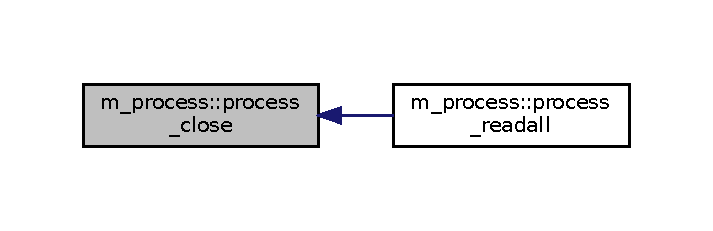
\includegraphics[width=342pt]{namespacem__process_ab4c5cad3fb46686f0c9b71c3a634f6ae_icgraph}
\end{center}
\end{figure}
\mbox{\Hypertarget{namespacem__process_a3c0f543a9ceff2671041d73660f60a59}\label{namespacem__process_a3c0f543a9ceff2671041d73660f60a59}} 
\index{m\_process@{m\_process}!process\_open@{process\_open}}
\index{process\_open@{process\_open}!m\_process@{m\_process}}
\doxysubsubsection{\texorpdfstring{process\_open()}{process\_open()}}
{\footnotesize\ttfamily subroutine, private m\+\_\+process\+::process\+\_\+open (\begin{DoxyParamCaption}\item[{character(len=$\ast$), intent(in)}]{cmd,  }\item[{character(len=$\ast$), intent(in)}]{mode,  }\item[{type(\mbox{\hyperlink{structm__process_1_1streampointer}{streampointer}}), intent(out)}]{fp,  }\item[{integer, intent(out)}]{ierr }\end{DoxyParamCaption})\hspace{0.3cm}{\ttfamily [private]}}

\hypertarget{namespacem__process_autotoc_md38}{}\doxysubsubsection{N\+A\+ME}\label{namespacem__process_autotoc_md38}
(L\+I\+C\+E\+N\+SE\+:PD) \hypertarget{namespacem__process_autotoc_md39}{}\doxysubsubsection{S\+Y\+N\+O\+P\+S\+IS}\label{namespacem__process_autotoc_md39}
\hypertarget{namespacem__process_autotoc_md40}{}\doxysubsubsection{D\+E\+S\+C\+R\+I\+P\+T\+I\+ON}\label{namespacem__process_autotoc_md40}
\hypertarget{namespacem__process_autotoc_md41}{}\doxysubsubsection{E\+X\+A\+M\+P\+LE}\label{namespacem__process_autotoc_md41}
\hypertarget{namespacem__process_autotoc_md42}{}\doxysubsubsection{A\+U\+T\+H\+OR}\label{namespacem__process_autotoc_md42}
John S. Urban \hypertarget{namespacem__process_autotoc_md43}{}\doxysubsubsection{L\+I\+C\+E\+N\+SE}\label{namespacem__process_autotoc_md43}
Public Domain 

References process\+\_\+debug.

Here is the caller graph for this function\+:\nopagebreak
\begin{figure}[H]
\begin{center}
\leavevmode
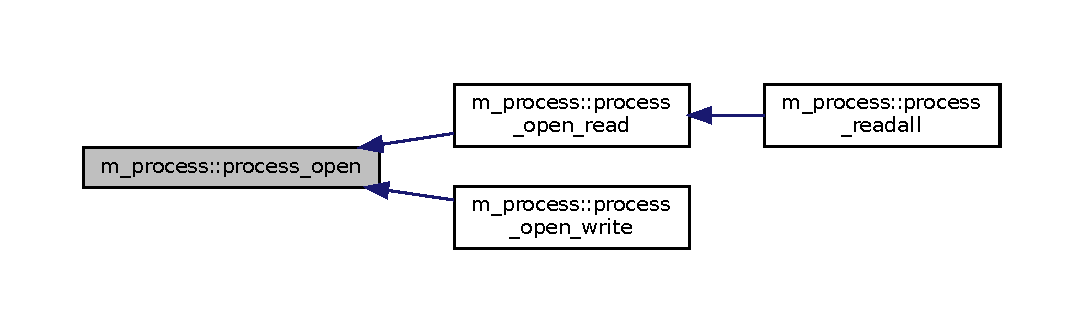
\includegraphics[width=350pt]{namespacem__process_a3c0f543a9ceff2671041d73660f60a59_icgraph}
\end{center}
\end{figure}
\mbox{\Hypertarget{namespacem__process_aaaf4d1926258a4cec7da7fc61c38c79d}\label{namespacem__process_aaaf4d1926258a4cec7da7fc61c38c79d}} 
\index{m\_process@{m\_process}!process\_open\_read@{process\_open\_read}}
\index{process\_open\_read@{process\_open\_read}!m\_process@{m\_process}}
\doxysubsubsection{\texorpdfstring{process\_open\_read()}{process\_open\_read()}}
{\footnotesize\ttfamily subroutine, public m\+\_\+process\+::process\+\_\+open\+\_\+read (\begin{DoxyParamCaption}\item[{character(len=$\ast$), intent(in)}]{cmd,  }\item[{type(\mbox{\hyperlink{structm__process_1_1streampointer}{streampointer}}), intent(out)}]{fp,  }\item[{integer, intent(out)}]{ierr }\end{DoxyParamCaption})}

\hypertarget{namespacem__process_autotoc_md22}{}\doxysubsubsection{N\+A\+ME}\label{namespacem__process_autotoc_md22}
process\+\_\+open\+\_\+read(3fm) -\/ \mbox{[}M\+\_\+process\mbox{]} open a process for reading using P\+O\+S\+IX interface (L\+I\+C\+E\+N\+SE\+:PD)\hypertarget{namespacem__process_autotoc_md23}{}\doxysubsubsection{S\+Y\+N\+O\+P\+S\+IS}\label{namespacem__process_autotoc_md23}
\begin{DoxyVerb} subroutine process_open_read(cmd,fp,ierr)

   character(len=*)    :: cmd
   type(streampointer) :: fp
   integer             :: ierr
\end{DoxyVerb}
\hypertarget{namespacem__process_autotoc_md24}{}\doxysubsubsection{D\+E\+S\+C\+R\+I\+P\+T\+I\+ON}\label{namespacem__process_autotoc_md24}
The M\+\_\+process Fortran procedures use the I\+S\+O\+\_\+\+C\+\_\+\+B\+I\+N\+D\+I\+NG interface to define Fortran-\/callable versions of the C procedures popen(3c)/pclose(3c) and fgets(3c)/fputs(3c). A set of record-\/oriented wrapper routines are then used to create a simple Fortran-\/callable interface.

A P\+O\+S\+IX C interface is generally available but may require using a Linux subwindow or an application such as Cyg\+Win on M\+S\+Windows platforms.

See \char`\"{}\+M\+\_\+process\char`\"{} for an extended description.\hypertarget{namespacem__process_autotoc_md25}{}\doxysubsubsection{O\+P\+T\+I\+O\+NS}\label{namespacem__process_autotoc_md25}
\begin{DoxyVerb}cmd      command passed to system to start process
fp       C file pointer returned by process_open_*()
ierr     error flag returned.

          o process_writeline(3f) : negative indicates an error
          o process_readline(3f)  : Non-zero indicates an error

maximum character value length is currently 4096
\end{DoxyVerb}
\hypertarget{namespacem__process_autotoc_md26}{}\doxysubsubsection{E\+X\+A\+M\+P\+L\+ES}\label{namespacem__process_autotoc_md26}
This example shows a routine to read the output of a system command.

program demo\+\_\+process\+\_\+open\+\_\+read use M\+\_\+process ,O\+N\+LY\+: process\+\_\+open\+\_\+read, process\+\_\+readline use M\+\_\+process ,O\+N\+LY\+: streampointer, process\+\_\+close implicit none type(streampointer) \+:: fp ! line of data to read (assumed long enough to hold any output line) character(len=4096) \+:: line integer \+:: ierr ! open process to read from call process\+\_\+open\+\_\+read(\textquotesingle{}ls -\/l\textquotesingle{},fp,ierr) write($\ast$,$\ast$)\textquotesingle{}R\+E\+A\+D\+T\+E\+ST\+: process is opened with status \textquotesingle{},ierr ierr=0 do while(ierr .eq. 0) ! read a line from the process call process\+\_\+readline(line,fp,ierr) if(ierr.\+ne.\+0)then write($\ast$,$\ast$)\textquotesingle{}R\+E\+A\+D\+T\+E\+ST\+: ierr is \textquotesingle{},ierr exit endif write($\ast$,$\ast$)\textquotesingle{}R\+E\+A\+D\+T\+E\+ST\+: \textquotesingle{},trim(line) enddo call process\+\_\+close(fp,ierr) write($\ast$,$\ast$)\textquotesingle{}R\+E\+A\+D\+T\+E\+ST\+: process closed with status \textquotesingle{},ierr end program demo\+\_\+process\+\_\+open\+\_\+read

Sample output\+:

R\+E\+A\+D\+T\+E\+ST\+: process is opened with status 0 R\+E\+A\+D\+T\+E\+ST\+: total 108 R\+E\+A\+D\+T\+E\+ST\+: -\/rw-\/r--r--. 1 urbanjs urbanjs 3731 Oct 17 14\+:49 build.\+sh R\+E\+A\+D\+T\+E\+ST\+: -\/rw-\/rw-\/r--. 1 urbanjs urbanjs 56633 Oct 17 14\+:50 build.\+sh.\+log R\+E\+A\+D\+T\+E\+ST\+: drwxrwxr-\/x. 3 urbanjs urbanjs 4096 Oct 17 14\+:50 doc R\+E\+A\+D\+T\+E\+ST\+: -\/rw-\/rw-\/r--. 1 urbanjs urbanjs 39459 Oct 17 15\+:16 M\+\_\+process.\+ff R\+E\+A\+D\+T\+E\+ST\+: -\/rw-\/rw-\/r--. 1 urbanjs urbanjs 826 Oct 17 15\+:17 xx.\+f90 R\+E\+A\+D\+T\+E\+ST\+: ierr is -\/1 R\+E\+A\+D\+T\+E\+ST\+: process closed with status 0\hypertarget{namespacem__process_autotoc_md27}{}\doxysubsubsection{S\+E\+E A\+L\+SO}\label{namespacem__process_autotoc_md27}
o P\+I\+P\+ES\+: pipe(3c), popen(3c), pclose(3c), fflush(3c) o N\+A\+M\+ED P\+I\+P\+ES\+: mkfifo(3c), mknod(3c) o S\+U\+B\+P\+R\+O\+C\+E\+S\+S\+ES\+: fork(3c) o O\+T\+H\+ER\+: fflush(3c) \hypertarget{namespacem__process_autotoc_md28}{}\doxysubsubsection{A\+U\+T\+H\+OR}\label{namespacem__process_autotoc_md28}
John S. Urban \hypertarget{namespacem__process_autotoc_md29}{}\doxysubsubsection{L\+I\+C\+E\+N\+SE}\label{namespacem__process_autotoc_md29}
Public Domain 

References process\+\_\+open().

Here is the call graph for this function\+:\nopagebreak
\begin{figure}[H]
\begin{center}
\leavevmode
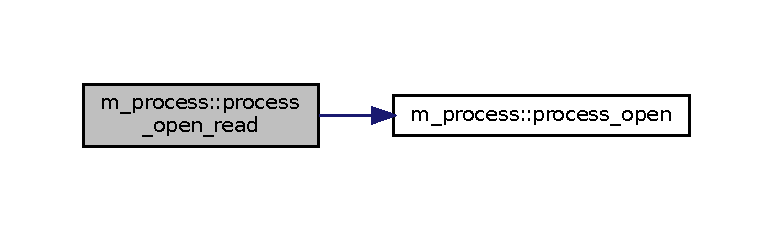
\includegraphics[width=350pt]{namespacem__process_aaaf4d1926258a4cec7da7fc61c38c79d_cgraph}
\end{center}
\end{figure}
Here is the caller graph for this function\+:\nopagebreak
\begin{figure}[H]
\begin{center}
\leavevmode
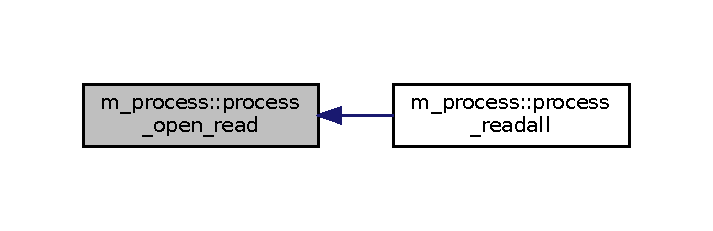
\includegraphics[width=342pt]{namespacem__process_aaaf4d1926258a4cec7da7fc61c38c79d_icgraph}
\end{center}
\end{figure}
\mbox{\Hypertarget{namespacem__process_aa6ed1404ab3472f5068ed15a7a01defc}\label{namespacem__process_aa6ed1404ab3472f5068ed15a7a01defc}} 
\index{m\_process@{m\_process}!process\_open\_write@{process\_open\_write}}
\index{process\_open\_write@{process\_open\_write}!m\_process@{m\_process}}
\doxysubsubsection{\texorpdfstring{process\_open\_write()}{process\_open\_write()}}
{\footnotesize\ttfamily subroutine, public m\+\_\+process\+::process\+\_\+open\+\_\+write (\begin{DoxyParamCaption}\item[{character(len=$\ast$), intent(in)}]{cmd,  }\item[{type(\mbox{\hyperlink{structm__process_1_1streampointer}{streampointer}}), intent(out)}]{fp,  }\item[{integer, intent(out)}]{ierr }\end{DoxyParamCaption})}

\hypertarget{namespacem__process_autotoc_md30}{}\doxysubsubsection{N\+A\+ME}\label{namespacem__process_autotoc_md30}
process\+\_\+open\+\_\+write(3fm) -\/ \mbox{[}M\+\_\+process\mbox{]} open a process for writing using a P\+O\+S\+IX interface (L\+I\+C\+E\+N\+SE\+:PD)\hypertarget{namespacem__process_autotoc_md31}{}\doxysubsubsection{S\+Y\+N\+O\+P\+S\+IS}\label{namespacem__process_autotoc_md31}
\begin{DoxyVerb} subroutine process_open_write(cmd,fp,ierr)

   character(len=*)    :: cmd
   type(streampointer) :: fp
   integer             :: ierr
\end{DoxyVerb}
\hypertarget{namespacem__process_autotoc_md32}{}\doxysubsubsection{D\+E\+S\+C\+R\+I\+P\+T\+I\+ON}\label{namespacem__process_autotoc_md32}
The M\+\_\+process Fortran procedures use the I\+S\+O\+\_\+\+C\+\_\+\+B\+I\+N\+D\+I\+NG interface to define Fortran-\/callable versions of the C procedures popen(3c)/pclose(3c) and fgets(3c)/fputs(3c). A set of record-\/oriented wrapper routines are then used to create a simple Fortran-\/callable interface.

A P\+O\+S\+IX C interface is generally available but may require using a Linux subwindow or an application such as Cyg\+Win on M\+S\+Windows platforms.

See \char`\"{}\+M\+\_\+process\char`\"{} for an extended description.\hypertarget{namespacem__process_autotoc_md33}{}\doxysubsubsection{O\+P\+T\+I\+O\+NS}\label{namespacem__process_autotoc_md33}
\begin{DoxyVerb}cmd      command passed to system to start process
fp       C file pointer returned by process_open_*()
ierr     error flag returned.

          o process_writeline(3f) : negative indicates an error
          o process_readline(3f)  : Non-zero indicates an error

maximum character value length is currently 4096
\end{DoxyVerb}
\hypertarget{namespacem__process_autotoc_md34}{}\doxysubsubsection{E\+X\+A\+M\+P\+L\+ES}\label{namespacem__process_autotoc_md34}
This example shows a routine to write lines to the stdin of a system process

program demo\+\_\+process\+\_\+open\+\_\+write use, intrinsic \+:: iso\+\_\+fortran\+\_\+env, only \+: \& \& stdin=$>$input\+\_\+unit, \& \& stdout=$>$output\+\_\+unit, \& \& stderr=$>$error\+\_\+unit use M\+\_\+process ,O\+N\+LY\+: process\+\_\+open\+\_\+write, \mbox{\hyperlink{interfacem__process_1_1process__writeline}{process\+\_\+writeline}} use M\+\_\+process ,O\+N\+LY\+: streampointer, process\+\_\+close implicit none type(streampointer) \+:: fp ! line of data to write character(len=4096) \+:: line integer \+:: ierr integer \+:: i ! open process to write to call process\+\_\+open\+\_\+write(\textquotesingle{}cat -\/n\textquotesingle{},fp,ierr) write(stdout,$\ast$)\textquotesingle{}O\+P\+E\+N\+W\+T\+E\+ST\+: process is opened with status \textquotesingle{},ierr ! remember C and Fortran I/O are often independent of each other flush(stdout) ierr=0 line=\textquotesingle{}xxxxxxxxxxxxxxxxxxxxxxxxxxx\textquotesingle{} do i=1,10 ! write a line to the process call process\+\_\+writeline(trim(line),fp,ierr) if(ierr.\+lt.\+0)then write(stdout,$\ast$)\textquotesingle{}O\+P\+E\+N\+W\+T\+E\+ST\+: ierr is \textquotesingle{},ierr exit endif enddo call process\+\_\+close(fp,ierr) write(stdout,$\ast$)\textquotesingle{}O\+P\+E\+N\+W\+T\+E\+ST\+: process closed with status \textquotesingle{},ierr end program demo\+\_\+process\+\_\+open\+\_\+write

Sample output\+:

$>$O\+P\+E\+N\+W\+T\+E\+ST\+: process is opened with status 0 \begin{quote}
1 xxxxxxxxxxxxxxxxxxxxxxxxxxx 2 xxxxxxxxxxxxxxxxxxxxxxxxxxx 3 xxxxxxxxxxxxxxxxxxxxxxxxxxx 4 xxxxxxxxxxxxxxxxxxxxxxxxxxx 5 xxxxxxxxxxxxxxxxxxxxxxxxxxx 6 xxxxxxxxxxxxxxxxxxxxxxxxxxx 7 xxxxxxxxxxxxxxxxxxxxxxxxxxx 8 xxxxxxxxxxxxxxxxxxxxxxxxxxx 9 xxxxxxxxxxxxxxxxxxxxxxxxxxx 10 xxxxxxxxxxxxxxxxxxxxxxxxxxx $>$O\+P\+E\+N\+W\+T\+E\+ST\+: process closed with status 0 \end{quote}
\hypertarget{namespacem__process_autotoc_md35}{}\doxysubsubsection{S\+E\+E A\+L\+SO}\label{namespacem__process_autotoc_md35}
o P\+I\+P\+ES\+: pipe(3c), popen(3c), pclose(3c), fflush(3c) o N\+A\+M\+ED P\+I\+P\+ES\+: mkfifo(3c), mknod(3c) o S\+U\+B\+P\+R\+O\+C\+E\+S\+S\+ES\+: fork(3c) o O\+T\+H\+ER\+: fflush(3c) \hypertarget{namespacem__process_autotoc_md36}{}\doxysubsubsection{A\+U\+T\+H\+OR}\label{namespacem__process_autotoc_md36}
John S. Urban \hypertarget{namespacem__process_autotoc_md37}{}\doxysubsubsection{L\+I\+C\+E\+N\+SE}\label{namespacem__process_autotoc_md37}
Public Domain 

References process\+\_\+open().

Here is the call graph for this function\+:\nopagebreak
\begin{figure}[H]
\begin{center}
\leavevmode
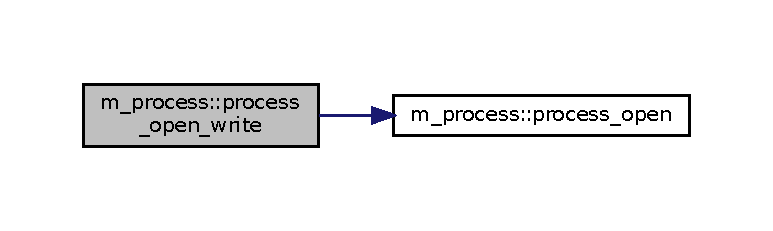
\includegraphics[width=350pt]{namespacem__process_aa6ed1404ab3472f5068ed15a7a01defc_cgraph}
\end{center}
\end{figure}
\mbox{\Hypertarget{namespacem__process_a7dd759a1344789477ae1e205d7fa9a51}\label{namespacem__process_a7dd759a1344789477ae1e205d7fa9a51}} 
\index{m\_process@{m\_process}!process\_readall@{process\_readall}}
\index{process\_readall@{process\_readall}!m\_process@{m\_process}}
\doxysubsubsection{\texorpdfstring{process\_readall()}{process\_readall()}}
{\footnotesize\ttfamily character(len=\+:) function, allocatable, public m\+\_\+process\+::process\+\_\+readall (\begin{DoxyParamCaption}\item[{character(len=$\ast$), intent(in)}]{cmd,  }\item[{character(len=$\ast$), intent(in), optional}]{delim,  }\item[{integer, intent(out), optional}]{ierr }\end{DoxyParamCaption})}

\hypertarget{namespacem__process_autotoc_md60}{}\doxysubsubsection{N\+A\+ME}\label{namespacem__process_autotoc_md60}
process\+\_\+readall(3f) -\/ \mbox{[}M\+\_\+process\mbox{]} read all lines from process into single string (L\+I\+C\+E\+N\+SE\+:PD) \hypertarget{namespacem__process_autotoc_md61}{}\doxysubsubsection{S\+Y\+N\+O\+P\+S\+IS}\label{namespacem__process_autotoc_md61}
syntax\+:

function process\+\_\+readall(cmd,delim,ierr) result(string)

character(len=$\ast$),intent(in) \+:: cmd character(len=$\ast$),intent(in),optional \+:: delim integer,intent(out),optional \+:: ierr character(len=\+:),allocatable \+:: string \hypertarget{namespacem__process_autotoc_md62}{}\doxysubsubsection{O\+P\+T\+I\+O\+NS}\label{namespacem__process_autotoc_md62}
cmd command to pass to system delim delimiter to place between output lines when they are concatenated. Defaults to a space ierr check status of call. \hypertarget{namespacem__process_autotoc_md63}{}\doxysubsubsection{R\+E\+S\+U\+L\+TS}\label{namespacem__process_autotoc_md63}
process\+\_\+readall Assuming sufficient memory is available all the output of the system command are concatenated into a string with spaces added between the output lines of the command. \hypertarget{namespacem__process_autotoc_md64}{}\doxysubsubsection{E\+X\+A\+M\+P\+LE}\label{namespacem__process_autotoc_md64}
Read all output of a command to a single string

program demo\+\_\+process\+\_\+readall use M\+\_\+process, only\+: process\+\_\+readall implicit none integer \+:: ierr character(len=\+:),allocatable \+:: string string=process\+\_\+readall(\textquotesingle{}ls\textquotesingle{},ierr=ierr) write($\ast$,$\ast$)ierr,string end program demo\+\_\+process\+\_\+readall

Results\+:

app build docs example fpm.\+toml L\+I\+C\+E\+N\+SE man R\+E\+A\+D\+M\+E.\+md src test

Read all output of a command to an array using split(3f)

program test\+\_\+process\+\_\+readall use M\+\_\+process ,only\+: process\+\_\+readall use M\+\_\+strings ,only\+: split implicit none integer \+:: ierr integer \+:: i character(len=\+:),allocatable \+:: string character(len=\+:),allocatable \+:: array(\+:) string=process\+\_\+readall(\textquotesingle{}ls\textquotesingle{},delim=N\+E\+W\+\_\+\+L\+I\+NE(\char`\"{}\+A\char`\"{}),ierr=ierr) call split(string,array,delimiters=N\+E\+W\+\_\+\+L\+I\+NE(\char`\"{}\+A\char`\"{})) do i=1,size(array) write($\ast$,\textquotesingle{}(i0,t10,\char`\"{}\mbox{[}\char`\"{},a,\char`\"{}\mbox{]}\char`\"{})\textquotesingle{})i,trim(array(i)) enddo write($\ast$,$\ast$)string=process\+\_\+readall(\& \& \textquotesingle{}ls\textquotesingle{},delim=N\+E\+W\+\_\+\+L\+I\+NE(\char`\"{}\+A\char`\"{}),ierr=ierr) write($\ast$,$\ast$)string end program test\+\_\+process\+\_\+readall

Results\+: \begin{DoxyVerb}> 1     [Articles]
> 2     [LIBRARY]
> 3     [PC]
> 4     [SHIP]
> 5     [SPEC]
> 6     [crib.dat]
> 7     [doc]
> 8     [html]
> 9     [index.html]
> 10    [plan.txt]
> 11    [questions]
> 12    [scripts]
> 13    [tmp]
\end{DoxyVerb}
\hypertarget{namespacem__process_autotoc_md65}{}\doxysubsubsection{S\+E\+E A\+L\+SO}\label{namespacem__process_autotoc_md65}
M\+\_\+process(3fm) \hypertarget{namespacem__process_autotoc_md66}{}\doxysubsubsection{A\+U\+T\+H\+OR}\label{namespacem__process_autotoc_md66}
John S. Urban \hypertarget{namespacem__process_autotoc_md67}{}\doxysubsubsection{L\+I\+C\+E\+N\+SE}\label{namespacem__process_autotoc_md67}
Public Domain 

References process\+\_\+close(), process\+\_\+open\+\_\+read(), and process\+\_\+readline().

Here is the call graph for this function\+:\nopagebreak
\begin{figure}[H]
\begin{center}
\leavevmode
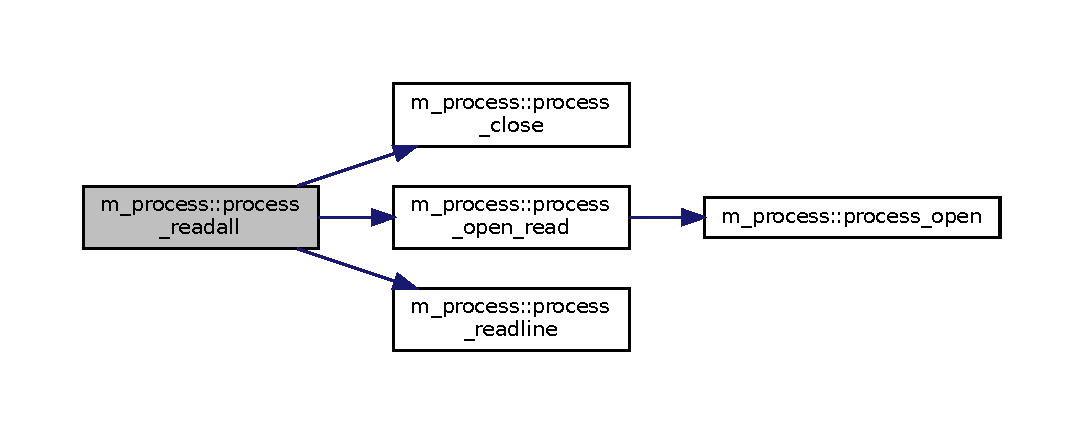
\includegraphics[width=350pt]{namespacem__process_a7dd759a1344789477ae1e205d7fa9a51_cgraph}
\end{center}
\end{figure}
\mbox{\Hypertarget{namespacem__process_acbc72c5ed371430a471aa1f3010fbbda}\label{namespacem__process_acbc72c5ed371430a471aa1f3010fbbda}} 
\index{m\_process@{m\_process}!process\_readline@{process\_readline}}
\index{process\_readline@{process\_readline}!m\_process@{m\_process}}
\doxysubsubsection{\texorpdfstring{process\_readline()}{process\_readline()}}
{\footnotesize\ttfamily subroutine, public m\+\_\+process\+::process\+\_\+readline (\begin{DoxyParamCaption}\item[{character(len=$\ast$), intent(out)}]{readfrom,  }\item[{type(\mbox{\hyperlink{structm__process_1_1streampointer}{streampointer}}), intent(in)}]{fp,  }\item[{integer, intent(out)}]{ierr }\end{DoxyParamCaption})}

\hypertarget{namespacem__process_autotoc_md52}{}\doxysubsubsection{N\+A\+ME}\label{namespacem__process_autotoc_md52}
process\+\_\+readline(3fm) -\/ \mbox{[}M\+\_\+process\mbox{]} read a line of output from a system command as a character variable (L\+I\+C\+E\+N\+SE\+:PD)\hypertarget{namespacem__process_autotoc_md53}{}\doxysubsubsection{S\+Y\+N\+O\+P\+S\+IS}\label{namespacem__process_autotoc_md53}
\begin{DoxyVerb} subroutine process_readline(string,fp,ierr)

   character(len=*)    :: string
   type(streampointer) :: fp
   integer             :: ierr
\end{DoxyVerb}
\hypertarget{namespacem__process_autotoc_md54}{}\doxysubsubsection{D\+E\+S\+C\+R\+I\+P\+T\+I\+ON}\label{namespacem__process_autotoc_md54}
The M\+\_\+process Fortran procedures use the I\+S\+O\+\_\+\+C\+\_\+\+B\+I\+N\+D\+I\+NG interface to define Fortran-\/callable versions of the C procedures popen(3c)/pclose(3c) and fgets(3c)/fputs(3c). A set of record-\/oriented wrapper routines are then used to create a simple Fortran-\/callable interface.

A P\+O\+S\+IX C interface is generally available but may require using a Linux subwindow or an application such as Cyg\+Win on M\+S\+Windows platforms.

See \char`\"{}\+M\+\_\+process\char`\"{} for an extended description.\hypertarget{namespacem__process_autotoc_md55}{}\doxysubsubsection{O\+P\+T\+I\+O\+NS}\label{namespacem__process_autotoc_md55}
\begin{DoxyVerb}string   data line to receive from process
fp       C file pointer returned by process_open_*()
ierr     error flag returned.

          o process_writeline(3f) : negative indicates an error
          o process_readline(3f)  : Non-zero indicates an error

maximum character value length is currently 4096
\end{DoxyVerb}
\hypertarget{namespacem__process_autotoc_md56}{}\doxysubsubsection{E\+X\+A\+M\+P\+L\+ES}\label{namespacem__process_autotoc_md56}
This example shows a routine reading the output of a system command.

program demo\+\_\+process\+\_\+readline use M\+\_\+process ,O\+N\+LY\+: process\+\_\+open\+\_\+read, process\+\_\+readline use M\+\_\+process ,O\+N\+LY\+: streampointer, process\+\_\+close implicit none type(streampointer) \+:: fp ! line of data to read (assumed long enough to hold any output line) character(len=4096) \+:: line integer \+:: ierr ! open process to read from call process\+\_\+open\+\_\+read(\textquotesingle{}ls -\/l\textquotesingle{},fp,ierr) write($\ast$,$\ast$)\textquotesingle{}R\+E\+A\+D\+L\+I\+NE\+: process is opened with status \textquotesingle{},ierr ierr=0 do while(ierr .eq. 0) ! read a line from the process call process\+\_\+readline(line,fp,ierr) if(ierr.\+ne.\+0)then write($\ast$,$\ast$)\textquotesingle{}R\+E\+A\+D\+L\+I\+NE\+: ierr is \textquotesingle{},ierr exit endif write($\ast$,$\ast$)\textquotesingle{}R\+E\+A\+D\+L\+I\+NE\+: \textquotesingle{},trim(line) enddo call process\+\_\+close(fp,ierr) write($\ast$,$\ast$)\textquotesingle{}R\+E\+A\+D\+L\+I\+NE\+: process closed with status \textquotesingle{},ierr end program demo\+\_\+process\+\_\+readline

Sample output\+:

R\+E\+A\+D\+L\+I\+NE\+: process is opened with status 0 R\+E\+A\+D\+L\+I\+NE\+: total 108 R\+E\+A\+D\+L\+I\+NE\+: -\/rw-\/r--r--. 1 urbanjs urbanjs 3731 Oct 17 14\+:49 build.\+sh R\+E\+A\+D\+L\+I\+NE\+: -\/rw-\/rw-\/r--. 1 urbanjs urbanjs 56633 Oct 17 14\+:50 build.\+sh.\+log R\+E\+A\+D\+L\+I\+NE\+: drwxrwxr-\/x. 3 urbanjs urbanjs 4096 Oct 17 14\+:50 doc R\+E\+A\+D\+L\+I\+NE\+: -\/rw-\/rw-\/r--. 1 urbanjs urbanjs 39459 Oct 17 15\+:16 M\+\_\+process.\+ff R\+E\+A\+D\+L\+I\+NE\+: -\/rw-\/rw-\/r--. 1 urbanjs urbanjs 826 Oct 17 15\+:17 xx.\+f90 R\+E\+A\+D\+L\+I\+NE\+: ierr is -\/1 R\+E\+A\+D\+L\+I\+NE\+: process closed with status 0\hypertarget{namespacem__process_autotoc_md57}{}\doxysubsubsection{S\+E\+E A\+L\+SO}\label{namespacem__process_autotoc_md57}
o P\+I\+P\+ES\+: pipe(3c), popen(3c), pclose(3c), fflush(3c) o N\+A\+M\+ED P\+I\+P\+ES\+: mkfifo(3c), mknod(3c) o S\+U\+B\+P\+R\+O\+C\+E\+S\+S\+ES\+: fork(3c) o O\+T\+H\+ER\+: fflush(3c) \hypertarget{namespacem__process_autotoc_md58}{}\doxysubsubsection{A\+U\+T\+H\+OR}\label{namespacem__process_autotoc_md58}
John S. Urban \hypertarget{namespacem__process_autotoc_md59}{}\doxysubsubsection{L\+I\+C\+E\+N\+SE}\label{namespacem__process_autotoc_md59}
Public Domain 

References process\+\_\+debug.

Here is the caller graph for this function\+:\nopagebreak
\begin{figure}[H]
\begin{center}
\leavevmode
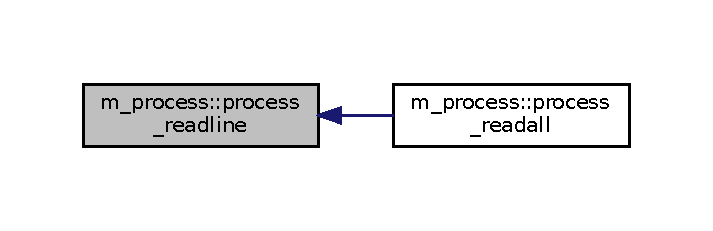
\includegraphics[width=342pt]{namespacem__process_acbc72c5ed371430a471aa1f3010fbbda_icgraph}
\end{center}
\end{figure}
\mbox{\Hypertarget{namespacem__process_a08887a918eba167ceacddf58ca084270}\label{namespacem__process_a08887a918eba167ceacddf58ca084270}} 
\index{m\_process@{m\_process}!process\_writeline\_array@{process\_writeline\_array}}
\index{process\_writeline\_array@{process\_writeline\_array}!m\_process@{m\_process}}
\doxysubsubsection{\texorpdfstring{process\_writeline\_array()}{process\_writeline\_array()}}
{\footnotesize\ttfamily subroutine m\+\_\+process\+::process\+\_\+writeline\+\_\+array (\begin{DoxyParamCaption}\item[{character(len=$\ast$), dimension(\+:), intent(in)}]{writefrom,  }\item[{type(\mbox{\hyperlink{structm__process_1_1streampointer}{streampointer}}), intent(in)}]{fp,  }\item[{integer, intent(out)}]{ierr }\end{DoxyParamCaption})\hspace{0.3cm}{\ttfamily [private]}}



References process\+\_\+debug, and process\+\_\+writeline\+\_\+scalar().

Here is the call graph for this function\+:\nopagebreak
\begin{figure}[H]
\begin{center}
\leavevmode
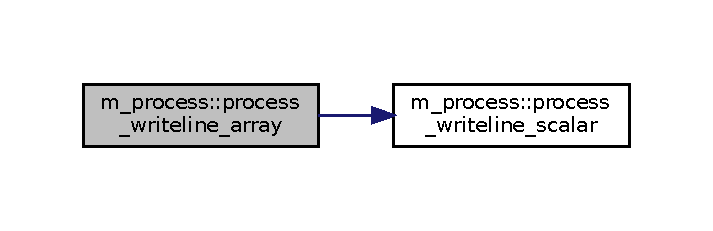
\includegraphics[width=342pt]{namespacem__process_a08887a918eba167ceacddf58ca084270_cgraph}
\end{center}
\end{figure}
\mbox{\Hypertarget{namespacem__process_a72527c0ec0af26dcb14b8bfad6dcd482}\label{namespacem__process_a72527c0ec0af26dcb14b8bfad6dcd482}} 
\index{m\_process@{m\_process}!process\_writeline\_scalar@{process\_writeline\_scalar}}
\index{process\_writeline\_scalar@{process\_writeline\_scalar}!m\_process@{m\_process}}
\doxysubsubsection{\texorpdfstring{process\_writeline\_scalar()}{process\_writeline\_scalar()}}
{\footnotesize\ttfamily subroutine m\+\_\+process\+::process\+\_\+writeline\+\_\+scalar (\begin{DoxyParamCaption}\item[{character(len=$\ast$), intent(in)}]{writefrom,  }\item[{type(\mbox{\hyperlink{structm__process_1_1streampointer}{streampointer}}), intent(in)}]{fp,  }\item[{integer, intent(out)}]{ierr,  }\item[{logical, intent(in), optional}]{trm }\end{DoxyParamCaption})\hspace{0.3cm}{\ttfamily [private]}}

\hypertarget{namespacem__process_autotoc_md68}{}\doxysubsubsection{N\+A\+ME}\label{namespacem__process_autotoc_md68}
process\+\_\+writeline(3fm) -\/ \mbox{[}M\+\_\+process\mbox{]} write to a process using a P\+O\+S\+IX interface (L\+I\+C\+E\+N\+SE\+:PD)\hypertarget{namespacem__process_autotoc_md69}{}\doxysubsubsection{S\+Y\+N\+O\+P\+S\+IS}\label{namespacem__process_autotoc_md69}
\begin{DoxyVerb} subroutine process_writeline(string,fp,ierr)

   character(len=*)    :: string
   type(streampointer) :: fp
   integer             :: ierr
\end{DoxyVerb}
\hypertarget{namespacem__process_autotoc_md70}{}\doxysubsubsection{D\+E\+S\+C\+R\+I\+P\+T\+I\+ON}\label{namespacem__process_autotoc_md70}
The M\+\_\+process Fortran procedures use the I\+S\+O\+\_\+\+C\+\_\+\+B\+I\+N\+D\+I\+NG interface to define Fortran-\/callable versions of the C procedures popen(3c)/pclose(3c) and fgets(3c)/fputs(3c). A set of record-\/oriented wrapper routines are then used to create a simple Fortran-\/callable interface.

A P\+O\+S\+IX C interface is generally available but may require using a Linux subwindow or an application such as Cyg\+Win on M\+S\+Windows platforms.

See \char`\"{}\+M\+\_\+process\char`\"{} for an extended description.\hypertarget{namespacem__process_autotoc_md71}{}\doxysubsubsection{O\+P\+T\+I\+O\+NS}\label{namespacem__process_autotoc_md71}
\begin{DoxyVerb}string   data line to to process
fp       C file pointer returned by process_open_*()
ierr     error flag returned.

          o process_writeline(3f) : negative indicates an error
          o process_readline(3f)  : Non-zero indicates an error

maximum character value length is currently 4096
\end{DoxyVerb}
\hypertarget{namespacem__process_autotoc_md72}{}\doxysubsubsection{E\+X\+A\+M\+P\+L\+ES}\label{namespacem__process_autotoc_md72}
This example shows a routine to write lines to the stdin of a system process

program demo\+\_\+process\+\_\+writeline use, intrinsic \+:: iso\+\_\+fortran\+\_\+env, only \+: \& \& stdin=$>$input\+\_\+unit, \& \& stdout=$>$output\+\_\+unit, \& \& stderr=$>$error\+\_\+unit use \mbox{\hyperlink{namespacem__process}{m\+\_\+process}} ,only\+: process\+\_\+open\+\_\+write, \mbox{\hyperlink{interfacem__process_1_1process__writeline}{process\+\_\+writeline}} use \mbox{\hyperlink{namespacem__process}{m\+\_\+process}} ,only\+: streampointer, process\+\_\+close implicit none type(streampointer) \+:: fp ! line of data to write character(len=4096) \+:: line integer \+:: ierr integer \+:: i ! open process to write to call process\+\_\+open\+\_\+write(\textquotesingle{}cat -\/n\textquotesingle{},fp,ierr) write($\ast$,$\ast$)\textquotesingle{}W\+R\+I\+T\+E\+T\+E\+ST\+: process is opened with status \textquotesingle{},ierr ! remember C and Fortran I/O are often independent of each other flush(stdout) ierr=0 line=\textquotesingle{}xxxxxxxxxxxxxxxxxxxxxxxxxxx\textquotesingle{} do i=1,10 ! write a line to the process call process\+\_\+writeline(trim(line),fp,ierr) if(ierr.\+lt.\+0)then write($\ast$,$\ast$)\textquotesingle{}W\+R\+I\+T\+E\+T\+E\+ST\+: ierr is \textquotesingle{},ierr exit endif enddo call process\+\_\+close(fp,ierr) write($\ast$,$\ast$)\textquotesingle{}W\+R\+I\+T\+E\+T\+E\+ST\+: process closed with status \textquotesingle{},ierr end program demo\+\_\+process\+\_\+writeline

Sample output\+:

$>$W\+R\+I\+T\+E\+T\+E\+ST\+: process is opened with status 0 \begin{quote}
1 xxxxxxxxxxxxxxxxxxxxxxxxxxx 2 xxxxxxxxxxxxxxxxxxxxxxxxxxx 3 xxxxxxxxxxxxxxxxxxxxxxxxxxx 4 xxxxxxxxxxxxxxxxxxxxxxxxxxx 5 xxxxxxxxxxxxxxxxxxxxxxxxxxx 6 xxxxxxxxxxxxxxxxxxxxxxxxxxx 7 xxxxxxxxxxxxxxxxxxxxxxxxxxx 8 xxxxxxxxxxxxxxxxxxxxxxxxxxx 9 xxxxxxxxxxxxxxxxxxxxxxxxxxx 10 xxxxxxxxxxxxxxxxxxxxxxxxxxx $>$W\+R\+I\+T\+E\+T\+E\+ST\+: process closed with status 0 \end{quote}
\hypertarget{namespacem__process_autotoc_md73}{}\doxysubsubsection{S\+E\+E A\+L\+SO}\label{namespacem__process_autotoc_md73}
o P\+I\+P\+ES\+: pipe(3c), popen(3c), pclose(3c), fflush(3c) o N\+A\+M\+ED P\+I\+P\+ES\+: mkfifo(3c), mknod(3c) o S\+U\+B\+P\+R\+O\+C\+E\+S\+S\+ES\+: fork(3c) o O\+T\+H\+ER\+: fflush(3c) \hypertarget{namespacem__process_autotoc_md74}{}\doxysubsubsection{A\+U\+T\+H\+OR}\label{namespacem__process_autotoc_md74}
John S. Urban \hypertarget{namespacem__process_autotoc_md75}{}\doxysubsubsection{L\+I\+C\+E\+N\+SE}\label{namespacem__process_autotoc_md75}
Public Domain 

References process\+\_\+debug.

Here is the caller graph for this function\+:\nopagebreak
\begin{figure}[H]
\begin{center}
\leavevmode
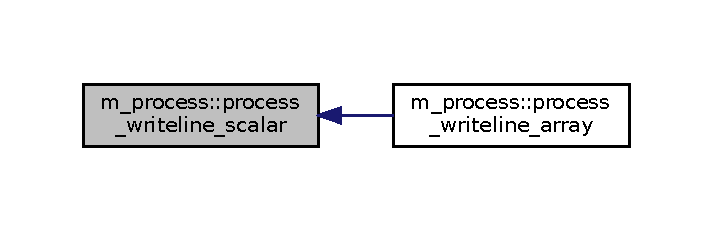
\includegraphics[width=342pt]{namespacem__process_a72527c0ec0af26dcb14b8bfad6dcd482_icgraph}
\end{center}
\end{figure}


\doxysubsection{Variable Documentation}
\mbox{\Hypertarget{namespacem__process_a0fabee8d01338d5523fbdea5c5f1e894}\label{namespacem__process_a0fabee8d01338d5523fbdea5c5f1e894}} 
\index{m\_process@{m\_process}!process\_debug@{process\_debug}}
\index{process\_debug@{process\_debug}!m\_process@{m\_process}}
\doxysubsubsection{\texorpdfstring{process\_debug}{process\_debug}}
{\footnotesize\ttfamily logical, public m\+\_\+process\+::process\+\_\+debug =.false.}


\chapter{Data Type Documentation}
\hypertarget{interfacem__process_1_1fflush}{}\section{m\+\_\+process\+:\+:fflush Interface Reference}
\label{interfacem__process_1_1fflush}\index{m\+\_\+process\+::fflush@{m\+\_\+process\+::fflush}}


\subsubsection*{N\+A\+ME}

fflush(3fp) -\/ flush buffered file output \subsubsection*{S\+Y\+N\+O\+P\+S\+IS} 


\subsection*{Private Member Functions}
\begin{DoxyCompactItemize}
\item 
integer(c\+\_\+int) function \mbox{\hyperlink{interfacem__process_1_1fflush_a77d0db933d548b3ee20b064e705a408e}{fflush}} (handle)
\end{DoxyCompactItemize}


\subsection{Detailed Description}
\subsubsection*{N\+A\+ME}

fflush(3fp) -\/ flush buffered file output \subsubsection*{S\+Y\+N\+O\+P\+S\+IS}

Syntax\+:

\#include $<$stdio.\+h$>$ int fflush(\+F\+I\+L\+E $\ast$\+F\+P); \subsubsection*{D\+E\+S\+C\+R\+I\+P\+T\+I\+ON}

The `stdio' output functions can buffer output before delivering it to the host system, in order to minimize the overhead of system calls.

Use `fflush' to deliver any such pending output (for the file or stream identified by FP) to the host system.

If FP is `N\+U\+LL', `fflush' delivers pending output from all open files.

Additionally, if FP is a seekable input stream visiting a file descriptor, set the position of the file descriptor to match next unread byte, useful for obeying P\+O\+S\+IX semantics when ending a process without consuming all input from the stream. R\+E\+T\+U\+R\+NS fflush returns \textquotesingle{}0\textquotesingle{} unless it encounters a write error; in that situation, it returns `E\+OF'. P\+O\+R\+T\+A\+B\+I\+L\+I\+TY A\+N\+SI C requires `fflush'. The behavior on input streams is only specified by P\+O\+S\+IX, and not all implementations follow P\+O\+S\+IX rules.

No supporting OS subroutines are required. 

\subsection{Constructor \& Destructor Documentation}
\mbox{\Hypertarget{interfacem__process_1_1fflush_a77d0db933d548b3ee20b064e705a408e}\label{interfacem__process_1_1fflush_a77d0db933d548b3ee20b064e705a408e}} 
\index{m\+\_\+process\+::fflush@{m\+\_\+process\+::fflush}!fflush@{fflush}}
\index{fflush@{fflush}!m\+\_\+process\+::fflush@{m\+\_\+process\+::fflush}}
\subsubsection{\texorpdfstring{fflush()}{fflush()}}
{\footnotesize\ttfamily integer(c\+\_\+int) function m\+\_\+process\+::fflush\+::fflush (\begin{DoxyParamCaption}\item[{type (c\+\_\+ptr), value}]{handle }\end{DoxyParamCaption})\hspace{0.3cm}{\ttfamily [private]}}



The documentation for this interface was generated from the following file\+:\begin{DoxyCompactItemize}
\item 
/home/urbanjs/venus/\+V600/github/\+M\+\_\+process/src/\mbox{\hyperlink{M__process_8f90}{M\+\_\+process.\+f90}}\end{DoxyCompactItemize}

\hypertarget{interfacem__process_1_1process__writeline}{}\section{m\+\_\+process\+:\+:process\+\_\+writeline Interface Reference}
\label{interfacem__process_1_1process__writeline}\index{m\+\_\+process\+::process\+\_\+writeline@{m\+\_\+process\+::process\+\_\+writeline}}
\subsection*{Private Member Functions}
\begin{DoxyCompactItemize}
\item 
subroutine \mbox{\hyperlink{interfacem__process_1_1process__writeline_a9e95166556bec54fd10568f01d02f34e}{process\+\_\+writeline\+\_\+scalar}} (writefrom, fp, ierr, trm)
\item 
subroutine \mbox{\hyperlink{interfacem__process_1_1process__writeline_aa3543e9b23056b2f35869003f777f65d}{process\+\_\+writeline\+\_\+array}} (writefrom, fp, ierr)
\end{DoxyCompactItemize}


\subsection{Member Function/\+Subroutine Documentation}
\mbox{\Hypertarget{interfacem__process_1_1process__writeline_aa3543e9b23056b2f35869003f777f65d}\label{interfacem__process_1_1process__writeline_aa3543e9b23056b2f35869003f777f65d}} 
\index{m\+\_\+process\+::process\+\_\+writeline@{m\+\_\+process\+::process\+\_\+writeline}!process\+\_\+writeline\+\_\+array@{process\+\_\+writeline\+\_\+array}}
\index{process\+\_\+writeline\+\_\+array@{process\+\_\+writeline\+\_\+array}!m\+\_\+process\+::process\+\_\+writeline@{m\+\_\+process\+::process\+\_\+writeline}}
\subsubsection{\texorpdfstring{process\+\_\+writeline\+\_\+array()}{process\_writeline\_array()}}
{\footnotesize\ttfamily subroutine m\+\_\+process\+::process\+\_\+writeline\+::process\+\_\+writeline\+\_\+array (\begin{DoxyParamCaption}\item[{character(len=$\ast$), dimension(\+:), intent(in)}]{writefrom,  }\item[{type(\mbox{\hyperlink{structm__process_1_1streampointer}{streampointer}}), intent(in)}]{fp,  }\item[{integer, intent(out)}]{ierr }\end{DoxyParamCaption})\hspace{0.3cm}{\ttfamily [private]}}

\mbox{\Hypertarget{interfacem__process_1_1process__writeline_a9e95166556bec54fd10568f01d02f34e}\label{interfacem__process_1_1process__writeline_a9e95166556bec54fd10568f01d02f34e}} 
\index{m\+\_\+process\+::process\+\_\+writeline@{m\+\_\+process\+::process\+\_\+writeline}!process\+\_\+writeline\+\_\+scalar@{process\+\_\+writeline\+\_\+scalar}}
\index{process\+\_\+writeline\+\_\+scalar@{process\+\_\+writeline\+\_\+scalar}!m\+\_\+process\+::process\+\_\+writeline@{m\+\_\+process\+::process\+\_\+writeline}}
\subsubsection{\texorpdfstring{process\+\_\+writeline\+\_\+scalar()}{process\_writeline\_scalar()}}
{\footnotesize\ttfamily subroutine m\+\_\+process\+::process\+\_\+writeline\+::process\+\_\+writeline\+\_\+scalar (\begin{DoxyParamCaption}\item[{character(len=$\ast$), intent(in)}]{writefrom,  }\item[{type(\mbox{\hyperlink{structm__process_1_1streampointer}{streampointer}}), intent(in)}]{fp,  }\item[{integer, intent(out)}]{ierr,  }\item[{logical, intent(in), optional}]{trm }\end{DoxyParamCaption})\hspace{0.3cm}{\ttfamily [private]}}



The documentation for this interface was generated from the following file\+:\begin{DoxyCompactItemize}
\item 
/home/urbanjs/venus/\+V600/github/\+M\+\_\+process/src/\mbox{\hyperlink{M__process_8f90}{M\+\_\+process.\+f90}}\end{DoxyCompactItemize}

\hypertarget{structm__process_1_1streampointer}{}\doxysection{m\+\_\+process\+::streampointer Type Reference}
\label{structm__process_1_1streampointer}\index{m\_process::streampointer@{m\_process::streampointer}}
\doxysubsection*{Public Attributes}
\begin{DoxyCompactItemize}
\item 
type(c\+\_\+ptr) \mbox{\hyperlink{structm__process_1_1streampointer_aaa577914dd36a5ef61670674dd3a194c}{handle}} = c\+\_\+null\+\_\+ptr
\end{DoxyCompactItemize}


\doxysubsection{Member Data Documentation}
\mbox{\Hypertarget{structm__process_1_1streampointer_aaa577914dd36a5ef61670674dd3a194c}\label{structm__process_1_1streampointer_aaa577914dd36a5ef61670674dd3a194c}} 
\index{m\_process::streampointer@{m\_process::streampointer}!handle@{handle}}
\index{handle@{handle}!m\_process::streampointer@{m\_process::streampointer}}
\doxysubsubsection{\texorpdfstring{handle}{handle}}
{\footnotesize\ttfamily type (c\+\_\+ptr) m\+\_\+process\+::streampointer\+::handle = c\+\_\+null\+\_\+ptr}



The documentation for this type was generated from the following file\+:\begin{DoxyCompactItemize}
\item 
/home/urbanjs/venus/\+V600/github/\+M\+\_\+process/src/\mbox{\hyperlink{M__process_8f90}{M\+\_\+process.\+f90}}\end{DoxyCompactItemize}

\hypertarget{interfacem__process_1_1system__fgets}{}\section{m\+\_\+process\+:\+:system\+\_\+fgets Interface Reference}
\label{interfacem__process_1_1system__fgets}\index{m\+\_\+process\+::system\+\_\+fgets@{m\+\_\+process\+::system\+\_\+fgets}}


\subsubsection*{N\+A\+ME}

fgets(3fp) -\/ get character string from a file or stream by calling fgets(3c) \subsubsection*{S\+Y\+N\+O\+P\+S\+IS} 


\subsection*{Private Member Functions}
\begin{DoxyCompactItemize}
\item 
type(c\+\_\+ptr) function \mbox{\hyperlink{interfacem__process_1_1system__fgets_a33f5f4ba1ea0fe4e0b757d7fa5e8a571}{system\+\_\+fgets}} (buf, siz, handle)
\end{DoxyCompactItemize}


\subsection{Detailed Description}
\subsubsection*{N\+A\+ME}

fgets(3fp) -\/ get character string from a file or stream by calling fgets(3c) \subsubsection*{S\+Y\+N\+O\+P\+S\+IS}

\#include $<$stdio.\+h$>$

char $\ast$fgets(char $\ast$\+B\+UF, int N, F\+I\+LE $\ast$\+FP); \subsubsection*{D\+E\+S\+C\+R\+I\+P\+T\+I\+ON}

Reads at most N-\/1 characters from FP until a newline is found. The characters including to the newline are stored in B\+UF. The buffer is terminated with a 0. \subsubsection*{R\+E\+T\+U\+R\+NS}

fgets(3c) returns the buffer passed to it, with the data filled in. If end of file occurs with some data already accumulated, the data is returned with no other indication. If no data are read, N\+U\+LL is returned instead. \subsubsection*{P\+O\+R\+T\+A\+B\+I\+L\+I\+TY}

Note that fgets(3c) returns all of the data, including the newline. 

\subsection{Constructor \& Destructor Documentation}
\mbox{\Hypertarget{interfacem__process_1_1system__fgets_a33f5f4ba1ea0fe4e0b757d7fa5e8a571}\label{interfacem__process_1_1system__fgets_a33f5f4ba1ea0fe4e0b757d7fa5e8a571}} 
\index{m\+\_\+process\+::system\+\_\+fgets@{m\+\_\+process\+::system\+\_\+fgets}!system\+\_\+fgets@{system\+\_\+fgets}}
\index{system\+\_\+fgets@{system\+\_\+fgets}!m\+\_\+process\+::system\+\_\+fgets@{m\+\_\+process\+::system\+\_\+fgets}}
\subsubsection{\texorpdfstring{system\+\_\+fgets()}{system\_fgets()}}
{\footnotesize\ttfamily type (c\+\_\+ptr) function m\+\_\+process\+::system\+\_\+fgets\+::system\+\_\+fgets (\begin{DoxyParamCaption}\item[{character(kind=c\+\_\+char), dimension($\ast$)}]{buf,  }\item[{integer(kind=c\+\_\+int), value}]{siz,  }\item[{type (c\+\_\+ptr), value}]{handle }\end{DoxyParamCaption})\hspace{0.3cm}{\ttfamily [private]}}



The documentation for this interface was generated from the following file\+:\begin{DoxyCompactItemize}
\item 
/home/urbanjs/venus/\+V600/github/\+M\+\_\+process/src/\mbox{\hyperlink{M__process_8f90}{M\+\_\+process.\+f90}}\end{DoxyCompactItemize}

\hypertarget{interfacem__process_1_1system__fputs}{}\doxysection{m\+\_\+process\+::system\+\_\+fputs Interface Reference}
\label{interfacem__process_1_1system__fputs}\index{m\_process::system\_fputs@{m\_process::system\_fputs}}
\doxysubsection*{Private Member Functions}
\begin{DoxyCompactItemize}
\item 
integer(c\+\_\+int) function \mbox{\hyperlink{interfacem__process_1_1system__fputs_a0a084cac4baf5058a79af7f6490c3a89}{system\+\_\+fputs}} (buf, handle)
\end{DoxyCompactItemize}


\doxysubsection{Detailed Description}
\hypertarget{interfacem__process_1_1system__fputs_autotoc_md14}{}\doxysubsubsection{N\+A\+ME}\label{interfacem__process_1_1system__fputs_autotoc_md14}
fputs(3fp) -\/ write a character string in a file or stream \hypertarget{interfacem__process_1_1system__fputs_autotoc_md15}{}\doxysubsubsection{S\+Y\+N\+O\+P\+S\+IS}\label{interfacem__process_1_1system__fputs_autotoc_md15}
\#include $<$stdio.\+h$>$

int fputs(const char $\ast$\+S, F\+I\+L\+E $\ast$\+F\+P);\hypertarget{interfacem__process_1_1system__fputs_autotoc_md16}{}\doxysubsubsection{D\+E\+S\+C\+R\+I\+P\+T\+I\+ON}\label{interfacem__process_1_1system__fputs_autotoc_md16}
`fputs' writes the string at S (but without the trailing null) to the file or stream identified by FP. R\+E\+T\+U\+R\+NS If successful, the result is `0'; otherwise, the result is `E\+OF'. P\+O\+R\+T\+A\+B\+I\+L\+I\+TY A\+N\+SI C requires `fputs', but does not specify that the result on success must be `0'; any non-\/negative value is permitted. 

\doxysubsection{Constructor \& Destructor Documentation}
\mbox{\Hypertarget{interfacem__process_1_1system__fputs_a0a084cac4baf5058a79af7f6490c3a89}\label{interfacem__process_1_1system__fputs_a0a084cac4baf5058a79af7f6490c3a89}} 
\index{m\_process::system\_fputs@{m\_process::system\_fputs}!system\_fputs@{system\_fputs}}
\index{system\_fputs@{system\_fputs}!m\_process::system\_fputs@{m\_process::system\_fputs}}
\doxysubsubsection{\texorpdfstring{system\_fputs()}{system\_fputs()}}
{\footnotesize\ttfamily integer(c\+\_\+int) function m\+\_\+process\+::system\+\_\+fputs\+::system\+\_\+fputs (\begin{DoxyParamCaption}\item[{character(kind=c\+\_\+char), dimension($\ast$)}]{buf,  }\item[{type (c\+\_\+ptr), value}]{handle }\end{DoxyParamCaption})\hspace{0.3cm}{\ttfamily [private]}}



The documentation for this interface was generated from the following file\+:\begin{DoxyCompactItemize}
\item 
/home/urbanjs/venus/\+V600/github/\+M\+\_\+process/src/\mbox{\hyperlink{M__process_8f90}{M\+\_\+process.\+f90}}\end{DoxyCompactItemize}

\hypertarget{interfacem__process_1_1system__pclose}{}\doxysection{m\+\_\+process\+::system\+\_\+pclose Interface Reference}
\label{interfacem__process_1_1system__pclose}\index{m\_process::system\_pclose@{m\_process::system\_pclose}}
\doxysubsection*{Private Member Functions}
\begin{DoxyCompactItemize}
\item 
integer(c\+\_\+int) function \mbox{\hyperlink{interfacem__process_1_1system__pclose_a8484cc191f8a18e155f97e284c3795ab}{system\+\_\+pclose}} (handle)
\end{DoxyCompactItemize}


\doxysubsection{Constructor \& Destructor Documentation}
\mbox{\Hypertarget{interfacem__process_1_1system__pclose_a8484cc191f8a18e155f97e284c3795ab}\label{interfacem__process_1_1system__pclose_a8484cc191f8a18e155f97e284c3795ab}} 
\index{m\_process::system\_pclose@{m\_process::system\_pclose}!system\_pclose@{system\_pclose}}
\index{system\_pclose@{system\_pclose}!m\_process::system\_pclose@{m\_process::system\_pclose}}
\doxysubsubsection{\texorpdfstring{system\_pclose()}{system\_pclose()}}
{\footnotesize\ttfamily integer(c\+\_\+int) function m\+\_\+process\+::system\+\_\+pclose\+::system\+\_\+pclose (\begin{DoxyParamCaption}\item[{type (c\+\_\+ptr), value}]{handle }\end{DoxyParamCaption})\hspace{0.3cm}{\ttfamily [private]}}



The documentation for this interface was generated from the following file\+:\begin{DoxyCompactItemize}
\item 
/home/urbanjs/venus/\+V600/github/\+M\+\_\+process/src/\mbox{\hyperlink{M__process_8f90}{M\+\_\+process.\+f90}}\end{DoxyCompactItemize}

\hypertarget{interfacem__process_1_1system__popen}{}\doxysection{m\+\_\+process\+::system\+\_\+popen Interface Reference}
\label{interfacem__process_1_1system__popen}\index{m\_process::system\_popen@{m\_process::system\_popen}}
\doxysubsection*{Private Member Functions}
\begin{DoxyCompactItemize}
\item 
type(c\+\_\+ptr) function \mbox{\hyperlink{interfacem__process_1_1system__popen_a45211cf49fdd755983b08ed6f3705bb1}{system\+\_\+popen}} (path, mode)
\end{DoxyCompactItemize}


\doxysubsection{Constructor \& Destructor Documentation}
\mbox{\Hypertarget{interfacem__process_1_1system__popen_a45211cf49fdd755983b08ed6f3705bb1}\label{interfacem__process_1_1system__popen_a45211cf49fdd755983b08ed6f3705bb1}} 
\index{m\_process::system\_popen@{m\_process::system\_popen}!system\_popen@{system\_popen}}
\index{system\_popen@{system\_popen}!m\_process::system\_popen@{m\_process::system\_popen}}
\doxysubsubsection{\texorpdfstring{system\_popen()}{system\_popen()}}
{\footnotesize\ttfamily type (c\+\_\+ptr) function m\+\_\+process\+::system\+\_\+popen\+::system\+\_\+popen (\begin{DoxyParamCaption}\item[{character(kind=c\+\_\+char), dimension($\ast$)}]{path,  }\item[{character(kind=c\+\_\+char), dimension($\ast$)}]{mode }\end{DoxyParamCaption})\hspace{0.3cm}{\ttfamily [private]}}



The documentation for this interface was generated from the following file\+:\begin{DoxyCompactItemize}
\item 
/home/urbanjs/venus/\+V600/github/\+M\+\_\+process/src/\mbox{\hyperlink{M__process_8f90}{M\+\_\+process.\+f90}}\end{DoxyCompactItemize}

\chapter{File Documentation}
\hypertarget{M__process_8f90}{}\section{/home/urbanjs/venus/\+V600/github/\+M\+\_\+process/src/\+M\+\_\+process.f90 File Reference}
\label{M__process_8f90}\index{/home/urbanjs/venus/\+V600/github/\+M\+\_\+process/src/\+M\+\_\+process.\+f90@{/home/urbanjs/venus/\+V600/github/\+M\+\_\+process/src/\+M\+\_\+process.\+f90}}
\subsection*{Data Types}
\begin{DoxyCompactItemize}
\item 
type \mbox{\hyperlink{structm__process_1_1streampointer}{m\+\_\+process\+::streampointer}}
\item 
interface \mbox{\hyperlink{interfacem__process_1_1process__writeline}{m\+\_\+process\+::process\+\_\+writeline}}
\item 
interface \mbox{\hyperlink{interfacem__process_1_1system__popen}{m\+\_\+process\+::system\+\_\+popen}}
\item 
interface \mbox{\hyperlink{interfacem__process_1_1system__fgets}{m\+\_\+process\+::system\+\_\+fgets}}
\begin{DoxyCompactList}\small\item\em \subsubsection*{N\+A\+ME}

fgets(3fp) -\/ get character string from a file or stream by calling fgets(3c) \subsubsection*{S\+Y\+N\+O\+P\+S\+IS}\end{DoxyCompactList}\item 
interface \mbox{\hyperlink{interfacem__process_1_1system__pclose}{m\+\_\+process\+::system\+\_\+pclose}}
\item 
interface \mbox{\hyperlink{interfacem__process_1_1system__fputs}{m\+\_\+process\+::system\+\_\+fputs}}
\begin{DoxyCompactList}\small\item\em \subsubsection*{N\+A\+ME}

fputs(3fp) -\/ write a character string in a file or stream \subsubsection*{S\+Y\+N\+O\+P\+S\+IS}\end{DoxyCompactList}\item 
interface \mbox{\hyperlink{interfacem__process_1_1fflush}{m\+\_\+process\+::fflush}}
\begin{DoxyCompactList}\small\item\em \subsubsection*{N\+A\+ME}

fflush(3fp) -\/ flush buffered file output \subsubsection*{S\+Y\+N\+O\+P\+S\+IS}\end{DoxyCompactList}\end{DoxyCompactItemize}
\subsection*{Modules}
\begin{DoxyCompactItemize}
\item 
module \mbox{\hyperlink{namespacem__process}{m\+\_\+process}}
\begin{DoxyCompactList}\small\item\em \subsubsection*{N\+A\+ME}

M\+\_\+process(3fm) -\/ \mbox{[}M\+\_\+process\mbox{]} Fortran Module for calling process-\/related C functions from Fortran (L\+I\+C\+E\+N\+SE\+:PD) \end{DoxyCompactList}\end{DoxyCompactItemize}
\subsection*{Functions/\+Subroutines}
\begin{DoxyCompactItemize}
\item 
subroutine, public \mbox{\hyperlink{namespacem__process_aaaf4d1926258a4cec7da7fc61c38c79d}{m\+\_\+process\+::process\+\_\+open\+\_\+read}} (cmd, fp, ierr)
\begin{DoxyCompactList}\small\item\em \subsubsection*{N\+A\+ME}

process\+\_\+open\+\_\+read(3fm) -\/ \mbox{[}M\+\_\+process\mbox{]} open a process for reading using P\+O\+S\+IX interface (L\+I\+C\+E\+N\+SE\+:PD) \end{DoxyCompactList}\item 
subroutine, public \mbox{\hyperlink{namespacem__process_aa6ed1404ab3472f5068ed15a7a01defc}{m\+\_\+process\+::process\+\_\+open\+\_\+write}} (cmd, fp, ierr)
\begin{DoxyCompactList}\small\item\em \subsubsection*{N\+A\+ME}

process\+\_\+open\+\_\+write(3fm) -\/ \mbox{[}M\+\_\+process\mbox{]} open a process for writing using a P\+O\+S\+IX interface (L\+I\+C\+E\+N\+SE\+:PD) \end{DoxyCompactList}\item 
subroutine, private \mbox{\hyperlink{namespacem__process_a3c0f543a9ceff2671041d73660f60a59}{m\+\_\+process\+::process\+\_\+open}} (cmd, mode, fp, ierr)
\begin{DoxyCompactList}\small\item\em \subsubsection*{N\+A\+ME}

(L\+I\+C\+E\+N\+SE\+:PD) \subsubsection*{S\+Y\+N\+O\+P\+S\+IS}\end{DoxyCompactList}\item 
subroutine, public \mbox{\hyperlink{namespacem__process_ab4c5cad3fb46686f0c9b71c3a634f6ae}{m\+\_\+process\+::process\+\_\+close}} (fp, ierr)
\begin{DoxyCompactList}\small\item\em \subsubsection*{N\+A\+ME}

process\+\_\+close(3fm) -\/ \mbox{[}M\+\_\+process\mbox{]} close a process being written to or read from (L\+I\+C\+E\+N\+SE\+:PD) \end{DoxyCompactList}\item 
subroutine, public \mbox{\hyperlink{namespacem__process_acbc72c5ed371430a471aa1f3010fbbda}{m\+\_\+process\+::process\+\_\+readline}} (readfrom, fp, ierr)
\begin{DoxyCompactList}\small\item\em \subsubsection*{N\+A\+ME}

process\+\_\+readline(3fm) -\/ \mbox{[}M\+\_\+process\mbox{]} read a line of output from a system command as a character variable (L\+I\+C\+E\+N\+SE\+:PD) \end{DoxyCompactList}\item 
character(len=\+:) function, allocatable, public \mbox{\hyperlink{namespacem__process_a7dd759a1344789477ae1e205d7fa9a51}{m\+\_\+process\+::process\+\_\+readall}} (cmd, delim, ierr)
\begin{DoxyCompactList}\small\item\em \subsubsection*{N\+A\+ME}

process\+\_\+readall(3f) -\/ \mbox{[}M\+\_\+process\mbox{]} read all lines from process into single string (L\+I\+C\+E\+N\+SE\+:PD) \subsubsection*{S\+Y\+N\+O\+P\+S\+IS}\end{DoxyCompactList}\item 
subroutine \mbox{\hyperlink{namespacem__process_a72527c0ec0af26dcb14b8bfad6dcd482}{m\+\_\+process\+::process\+\_\+writeline\+\_\+scalar}} (writefrom, fp, ierr, trm)
\begin{DoxyCompactList}\small\item\em \subsubsection*{N\+A\+ME}

process\+\_\+writeline(3fm) -\/ \mbox{[}M\+\_\+process\mbox{]} write to a process using a P\+O\+S\+IX interface (L\+I\+C\+E\+N\+SE\+:PD) \end{DoxyCompactList}\item 
subroutine \mbox{\hyperlink{namespacem__process_a08887a918eba167ceacddf58ca084270}{m\+\_\+process\+::process\+\_\+writeline\+\_\+array}} (writefrom, fp, ierr)
\end{DoxyCompactItemize}
\subsection*{Variables}
\begin{DoxyCompactItemize}
\item 
logical, public \mbox{\hyperlink{namespacem__process_a0fabee8d01338d5523fbdea5c5f1e894}{m\+\_\+process\+::process\+\_\+debug}} =.false.
\end{DoxyCompactItemize}

\hypertarget{mainpage_8txt}{}\section{/home/urbanjs/venus/\+V600/github/\+M\+\_\+process/src/mainpage.txt File Reference}
\label{mainpage_8txt}\index{/home/urbanjs/venus/\+V600/github/\+M\+\_\+process/src/mainpage.\+txt@{/home/urbanjs/venus/\+V600/github/\+M\+\_\+process/src/mainpage.\+txt}}

%--- End generated contents ---

% Index
\backmatter
\newpage
\phantomsection
\clearemptydoublepage
\addcontentsline{toc}{chapter}{Index}
\printindex

\end{document}
